\documentclass[a4paper, 11pt]{book}
\usepackage{geometry}


\usepackage[utf8]{inputenc} 
\usepackage{fontspec} 
\usepackage{amsmath}
\usepackage{amssymb}
\usepackage{enumitem}
\usepackage{longtable}

% Bibliography
\usepackage{biblatex} 
\usepackage[hidelinks]{hyperref} \addbibresource{bibliography.bib}

% Listings
\usepackage{float} 
\usepackage{listings} \newfloat{lstfloat}{htbp}{lop} \floatname{lstfloat}{Listing} 
\def\lstfloatautorefname{Listing}

% Graphics
\usepackage{tikz}
\graphicspath{ {./img/} }

% Comments
\newcommand{\comment}[1]{} 

\title{Efficient GPU Implementation of Stencils on Unstructured Grids} 
\author{André Rösti}

\begin{document}

\newgeometry{centering}
\begin{titlepage}
	\begin{center}
		\vspace*{2cm}
		{\Huge \textbf{Efficient GPU Implementation of Stencils on Unstructured Grids}}
		\vspace{2cm}
		
		{\Large \textit{Bachelor Thesis}}
		\vspace{2cm}
		
		André Albert Rösti
		
		May 14, 2020
	\end{center}
	\vfill
	\raggedleft Advisors: Dr. T. Gysi, Dr. T. Grosser, Prof. T. Hoefler
		
	\raggedleft Department of Computer Science, ETH Zürich
	\vspace*{2cm}
\end{titlepage}
\restoregeometry

\thispagestyle{empty}

\pagenumbering{roman}
\tableofcontents

\chapter*{Abstract}

Stencil computations on unstructured grids with a regular Z-dimension are frequently performed in meteorology for atmospheric modeling. While using a GPU to parallelize execution of such stencils promises fast runtimes, supporting the irregular structure in two dimensions complicates their implementation, as neighborship access necessitates indirect memory lookups.

In this thesis, we explore various approaches of storing unstructured grids with one regular dimension and accessing them from the GPU in a stencil computation. We benchmark the performance of three real-world stencils of varying complexity on various unstructured grid implementations, some of which make explicit use of the Z-regularity. In our initial naive approaches, we observe slowdowns of $122\%$ (simple stencil), $52\%$ (medium-complexity stencil), and $5\%$ (complex stencil) compared to executing the same stencils on entirely regular grids. Notably, through a neighborship table compression scheme, we are able to improve those values to $49\%$, $30\%$ and $5\%$ (no improvement) respectively. Other optimizations are explored. We also detail the foundations of the Nvidia CUDA GPU architecture.

\chapter*{Introduction}

Weather prediction is a challenging task to computers. A large number of factors, drawn from large data sets, interact in ways governed by complex physical equations. In order to solve the governing equations of the atmosphere, the computations are discretized on grids spanning the globe (or some local segment of it). Methods such as the \emph{finite differences} and \emph{finite volume} method solve these equations by performing (simple) calculations on each cell that depend only on a limited neighborhood of that cell. This type of computation, called a \emph{stencil}, can be implemented efficiently on graphics processing units, which provide a massively parallel architecture. 

Needless to say, a weather prediction computation for some instant in the future is only useful if the computation terminates before that point in time. Therefore, performance is a critical aspect of any application in weather prediction. The desire for more accurate results, on the other hand, opposes fast runtimes.

More fine-grained grids provide more accurate results but naturally lead to higher data traffic and slower runtimes. So-called \emph{unstructured grids} provide a compromise between globally coarse and globally fine-grained regular grids. Unstructured grids enable higher resolutions in areas of interest while other areas which require less detail can be covered by larger cells. Because of their ineherent irregularities, however, unstructured grids add an aditional overhead. Finding the location of neighboring cells' values especially becomes more involved, requiring additional memory lookups.

The main aim of this thesis is to contrast stencil performance in regular and unstructured grids, as well as exploring some means of optimization. The discrete approximations of the atmosphere's equations are of low arithmetic intensity -- the computations performed on each cell are simple. However, the operations performed are very memory-bandwith hungry, as each cell requires a lot of input data (several neighboring cells). Thus data locality greatly aids performance. The major focus of this report thus lies in evaluating different memory access strategies and schemes for optimizing the neighborship lookups in unstructured grids for three selected stencils.

In the following sections, we first explain the characteristics of grids and stencils in more detail and elaborate on the architecture of GPUs, on which these stencil calculations are performed. We continue by showing our purused methods of implementing regular and unstructured grid memory layouts and show different unoptimized and optimized means of accessing grid elements in stencil computations from the GPU. In section \ref{sec:results}, we finally present the observed overhead that the use of unstructured grids imposed when calculating identical stencils on identical data.
\chapter{Related Work}

Solano-Quinde et al. \cite{solano2011} present an algorithm for implementing scientific analyses in unstructured grids on GPUs for more general problems. They identify occupancy and memory access as the main limiting factors of performance. Their paper also explores the implications of using different memory layouts for the unstructured grid representation, arriving at the conclusion that struct-of-array-type layouts (see also section \ref{sec:representing-multiple-fields} in this report) are better suited for GPUs because of coalescing concerns. 

In this report, we assume the unstructured grid on top of which to apply a stencil is already given. An overview of the various methods of how such grids can be generated is given in \cite{mavriplis1997}. Section 3.4 of the publication also briefly hints at how an unstructured grid may be stored. This forms the basis of our initial naive storage approach.

A lot of research has been carried out concerning the compressed storage of meshes \cite{edgebreaker}\cite{edgebreaker-quadrilateral}. However, most of those approaches are not applicable to our problem, where decompression has to be virtually free and reordering of values is not permittable. The approach presented for compressing social network graphs in \cite{social} is similar to our compression approach.

\pagenumbering{arabic}
\chapter{Background}                                    \label{sec:foundations}

In this chapter, we introduce the terms and definitions that form the basis for the rest of the thesis. Specifically, we introduce \emph{regular} and \emph{unstructured grids}, \emph{stencils} and surrounding terminology (\emph{coordinates}, \emph{indices}, \emph{halo}) in sections \ref{sec:grids} and \ref{sec:stencils}. We then move to a discussion of parallel programming using the Nvidia \emph{CUDA} programming model \ref{sec:cuda-basics}, including a description of the memory hierarchy and performance metrics.

\section{Grids}                                            \label{sec:grids}

A grid partitions (tessellates) some space into a discrete number of cells. In weather/climate modeling, the three-dimensional space of the atmosphere is subdivided by a grid to facilitate finding numerical solutions to equations governing the weather. Each cell may contain one or multiple values (\emph{fields}) such as the temperature or humidity at a location.

One kind of grid is the \emph{regular grid}. In this type of \emph{structured grid}, each cell is of uniform size and has a fixed amount of six direct neighbors (top, bottom, left, right, front, and back). Real-life objects that have the structure of a regular grid are checkerboards (two dimensions) or a Rubik's cube (three dimensions). Because of their regularity, storing such grids in memory is straightforward.

In certain use cases, the use of \emph{unstructured grids} is beneficial to the requirements of the application at hand. In contrast to regular grids, cells need not be of equal size in unstructured grids and may have a varying number of neighbors. This means that the location of a cell's neighbor in memory no longer follows a regular structure. Because neighbor's locations are no longer inherently clear, an unstructured grid requires a neighborship table to describe its structure. Accessing a neighbor requires an indirect memory lookup in order to determine its location in memory.

This thesis is concerned with the performance implications that porting a stencil computation from a regular to an unstructured grid entails. It compares the cost indirect addressing imposes upon several different widely-used stencils.

While an unstructured grid theoretically supports arbitrary neighborship relations, for this thesis, we restrict irregularities to the X-Y-plane and assume even unstructured grids are regular (i.e. always have at most two neighbors) in the Z-dimension. This is a common use case in atmospheric modeling applications. In practice, such as in so-called \emph{icosahedral grids}, most of the neighborships in the X-Y-plane will also most often have some structure to it. We make use of these regularities in the optimizations described in section \ref{sec:grid-implementations} and \ref{sec:optimizations}.


\subsection{Coordinates and Indices}

In our implementations, cells in a grid are identified by \emph{coordinates}, which relate a cell to its real-world position and \emph{indices} which give the storage location of a cell in memory. 

Throughout the rest of this report we refer to the size of a grid as the \emph{maximum number of elements} in each dimension, and denote it by the vector
$$d = \begin{pmatrix}d_x \\ d_y \\ d_z\end{pmatrix}.$$
A unique identifier for each cell on the grid is given by its coordinates, denoted in similar fashion by a vector
$$p = \begin{pmatrix}p_x \\ p_y \\ p_z\end{pmatrix}.$$
The coordinates correspond to a position in Euclidian space. Coordinates are chosen such that each integer coordinate maps \emph{uniquely} to at most one cell. The converse (i.e. each cell has only one coordinate) is only true in regular grids: In the regular grid, direct adjacent cells differ in exactly one coordinate by an amount of one. In unstructured grids, not every coordinate is necessarily assigned to any cell, and one cell may span multiple coordinates. Therefore, an unstructured cell's neighbor might have coordinates that differ by more than one in multiple components.

As memory is one-dimensional, a mapping from the three-dimensional coordinates of a cell to its location in memory is required of a grid implementation. We call this location in memory the \emph{index} and denote it with the letter $i$. The mapping from three-dimensional coordinate space to the one-dimensional memory index defines the memory layout of the grid. In regular grids, this mapping is straightforward, while in unstructured grids it may be arbitrary. How regular and unstructured grids are laid out in memory is detailed in section \ref{sec:grid-implementations}.

\section{Stencils}                                    \label{sec:stencils}

Finding approximate numerical solutions to the governing equations of physical processes, as in meteorology, often entails performing certain unchanging calculations on every cell of a grid. The result of this process is again a grid of similar size. For each cell, the calculated output value is dependent only on a bounded small number of neighboring cells' values (\emph{neighborhood}). Such a computation is called \emph{stencil}. Simple stencils may require only the values of the current cell as well as directly adjacent (face-touching) neighbors in order to calculate the output value, while more complex ones could also depend on diagonal neighbors, neighbors-of-neighbors, etc. Yet, some spatial locality is guaranteed. 

\paragraph{Halo} \label{sec:halo} In stencil computations, special consideration needs to be given to the boundary cells of the grid. Compared to cells in the grid's interior, cells at the edges of the grid lack some neighbors. As such, the output value of a stencil that depends on these neighbors is undefined at the affected boundary cells. One way to address this issue is to execute the stencil only on the safe interior of the grid, separated from the boundary by a certain amount of padding. The amount of padding used depends on the size of the neighborhood which the stencil requires for its computation.

We call the set of cells residing in the padding around the boundaries of the grid \emph{halo}. Stencil implementations may include a branch instruction that prevents any computations if a cell lies in the halo. Alternatively, for ease of implementation and performance, it can be beneficial to store the halo separately in memory.

\section{GPU Programming on the Nvidia CUDA Platform} 	\label{sec:cuda-basics}

\emph{Graphics processing units} (GPUs) particularly lend themselves to stencil computations. In this section, we contrast the execution model of classical \emph{central processing units} (CPUs) with that of GPUs. We explain why stencil applications can profit from execution on the GPU and elaborate on the fundamentals of the \emph{Nvidia CUDA} platform for execution on the GPU.

Most classical computer programs run sequentially on the CPU. Computations are performed step-by-step. Such a sequence of operations is called \emph{thread}. Early CPUs were only capable of running one thread at a time. Even today, only a handful of threads (i.e. execution streams) can run truly in parallel on a CPU. Operating on large data sets on the CPU therefore still mostly involves repeated calculations within loops that handle one data point at a time.

Most performance optimizations in CPUs target \emph{latency}; caches, pipelining, branch prediction, and similar techniques aim to reduce the time between issuing a command and storing its result. While CPUs have become much faster since their inception, the improvements to performance have recently slowed due to physical constraints.

Sustained demands for faster runtimes and more complex applications have thus forced rethinking the sequential execution model. Many real-world applications on large data sets consist of largely unvarying computations on many data points. These applications often have few sequential dependencies. Applications in computer graphics, for example, often entail highly monotone computations that are repeated for every pixel displayed on the screen. The resulting value of the pixel at one edge of the screen often does not require knowledge of the result of a pixel at the other end, but sequential execution still dictates one value being calculated before the other. GPUs overcome the performance limits of sequential computation by providing thousands of hardware units which are able to compute (run threads) independently from one another, at the same time. \cite[Chapter~2]{cuda-for-engineers} This increases the \emph{throughput} of those devices: While a \emph{low-latency} CPU reacts to an issued command fast, it provides only one result for one data point. Meanwhile, a \emph{high throughput} GPU might take a longer time to issue the command, but it calculates the results for several datapoints ``at once''.

CPUs, therefore, shine in scenarios where calculations are less straightforward and predictable, while GPUs are more useful wherever monotone computations on large data sets are performed. Another advantage of GPUs is \emph{scalability}: Because the performed parallel computations are completely independent, larger problem sizes can effectively be solved more efficiently simply by adding more parallel execution capabilities to the hardware, i.e. adding more processors. 

Despite the name, GPUs are today no longer just used for graphics processing. Such computing is also called general-purpose GPU programming, or GPGPU for short.

The task of applying a stencil to a grid (sections \ref{sec:grids}, \ref{sec:stencils}) greatly benefits in terms of performance from execution on highly parallel architectures such as graphics processing units (\emph{GPUs}), as it can easily be parallelized by decomposing the problem domain. Each thread may be responsible for calculating the result of one cell or a small set of cells in the output grid. As data dependencies are limited to a local neighborhood, parallel threads can work on spatially separated data concurrently without risk of data races in most cases. Data races only occur if threads share some dependencies, i.e. when their neighborhood overlaps. In that case, each thread can re-compute its dependencies (called \emph{computation on-the-fly}) or threads may share their results by means of \emph{synchronization}.

In this thesis, we use the \emph{Nvidia CUDA} architecture to implement meteorological stencil computations on the \emph{Nvidia Tesla V100} GPU, and we assess their performance on different types of grids.

\subsection{SIMT Execution Model}

\emph{CUDA} employs a \emph{Single Instruction, Multiple Thread (SIMT)} execution model. This model can be compared to the \emph{Single Instruction, Multiple Data (SIMD)} model but makes writing programs more straight-forward to programmers experienced in sequential programming. \cite[Section~3.1]{ptx-isa} 

In a \emph{SIMD} model, instructions are ``wide'': They support input operands that are larger than single scalar values. Programmers explicitly issue these \emph{vector instructions} to perform a calculation on a set of values. In contrast, in the SIMT model used by \emph{CUDA}, programmers do not need to explicitly perform operations on multiple data points. Instead, code is written such that it operates on single scalar values. Many instances, i.e. \emph{threads}, of this code are run which differ only in an input \emph{thread index} they receive as input. In most applications, this input is used to determine which data point the thread operates on. Upon execution, when the same operation is executed in many threads on consecutive data points, they are grouped together automatically to be executed in parallel in SIMD-like fashion.

\subsection{Software}

Code to be executed on the GPU is written in specially-annotated functions called \emph{kernels}. Kernels can be written as regular C code but are compiled by the distinct Nvidia compiler \emph{(nvcc)} to \emph{Parallel Thread Execution (PTX)} machine code which can be run on the GPU. Inside a kernel, a \emph{thread and block index} is made available. Using a special syntax recognized by \emph{nvcc}, kernels can be launched from the CPU onto the GPU (sometimes simply called \emph{device}, as opposed to \emph{host} which refers to the CPU). The \emph{CUDA} Application Programming Interface (API) provides a device synchronization routine, which is required to synchronize CPU and GPU after the computation of the kernel on the GPU is completed. This enables relatively simple offloading of parallelizable workloads onto the GPU as a coprocessor while continuing to run the rest of the program asynchronously on the CPU. The \emph{CUDA} API furthermore provides routines for memory allocation on the device, memory prefetching (see \ref{sec:unified-memory} unified memory), and setting certain device parameters.

\begin{lstfloat}
\begin{lstlisting}[caption={Example showing kernel, its launch and CUDA API calls for allocating unified memory},captionpos=b,language=C]
// Kernel Definition. This function runs on the GPU.
__global__
void multiply(double fac, double *input, double *output) {
    int i = threadIdx.x + blockIdx.x*blockDim.x;
    output[i] = fac * input[i];
}

// Kernel Invocation. This function runs on the CPU.
int main(int argc, char **argv) {
    double *input, output;
    int N = 1024 * 1024;
    cudaMallocManaged(&input, N * sizeof(double));
    cudaMallocManaged(&output, N * sizeof(double));
    cudaMemset(input, 42.0, N * sizeof(double));
    multiply<<<N/256, 256>>>(3.0, input, output);
    cudaDeviceSynchronize();
    cudaFree(input);
    cudaFree(output);
}
\end{lstlisting}
\end{lstfloat}

\subsection{Streaming Multiprocessors} \label{sec:hardware}

\emph{CUDA}-capable GPUs are structured as an array of so-called \emph{Streaming Multiprocessors (SMs)}. Each SM contains a multitude of scalar processor cores. These cores include arithmetic, logic, and floating-point units (ALUs, FPUs) and perform the actual computations on the data points. Together, they are used to advance computation in a \emph{warp}. A warp is a set of (typically 32) threads that are executed concurrently on the same multiprocessor. In every cycle, each thread inside a warp either uses one of the scalar cores to execute the same instruction as the other threads (on different data), or it is turned off if a branch diverged previously. A warp of multiple threads at the same instruction pointer executing the same instruction is therefore similar to executing a SIMD instruction on multiple data points.

Each SM has its own scheduler and operates completely independently of the other SMs. If the threads inside a warp diverge (because of branching instructions), the different execution paths are executed sequentially on the SM. It is therefore paramount to performance that kernels are written in such a way that threads in the same warp follow the same execution path whenever possible. One way to achieve this is to ensure branch conditions involve only the thread index divided by 32 (the warp size), as this will be the same value for all threads inside a warp. 

SMs choose the threads to form a warp from a pool of threads called a \emph{block}. When one warp finishes executing or is stalled (e.g. because of a memory dependency), the next set of threads forming a warp in the block is chosen to be executed. All threads in a block execute on the same SM. Resources such as registers and shared memory are divided among all threads in a block. Threads in the same block can communicate with one another through so-called \emph{shared memory}. Using the \texttt{\_\_syncthreads()} command in a kernel synchronizes all threads in the same block.

When a kernel is launched, the programmer may specify how many threads should be part of the same block (\emph{block size}), and how many blocks there should be (\emph{grid size}). These parameters are called the \emph{launch configuration}. It is important to have more blocks than SMs, as otherwise, some SMs will have no work to perform. Furthermore, if a synchronization instruction is used in the kernel, it is beneficial to have multiple blocks per SM, as to occupy the SM when one of the blocks is stalling because it is waiting for synchronization. The number of threads per block (block size) should be a multiple of 32 to ensure warps can be entirely filled with threads. \cite[Section~10]{cuda-best-practices}

\subsection{Memories} \label{sec:memories}

\begin{figure}
    \makebox[\textwidth][c]{
    


\tikzset{every picture/.style={line width=0.75pt}} %set default line width to 0.75pt        

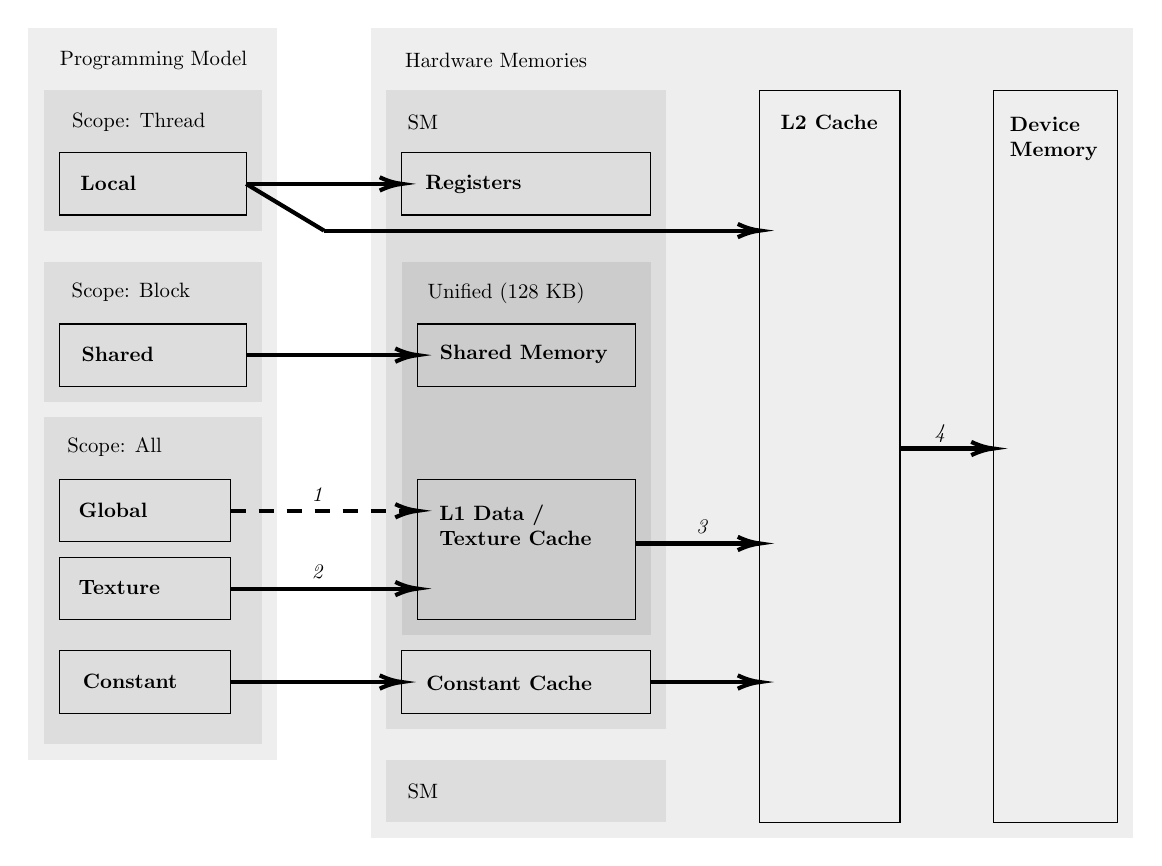
\begin{tikzpicture}[x=0.75pt,y=0.75pt,yscale=-0.75,xscale=0.75, every node/.style={scale=0.75}]
%uncomment if require: \path (0,574); %set diagram left start at 0, and has height of 574

%Shape: Rectangle [id:dp49466026838319044] 
\draw  [draw opacity=0][fill={rgb, 255:red, 238; green, 238; blue, 238 }  ,fill opacity=1 ] (10,10) -- (170,10) -- (170,480) -- (10,480) -- cycle ;
%Shape: Rectangle [id:dp28817003892392545] 
\draw  [draw opacity=0][fill={rgb, 255:red, 221; green, 221; blue, 221 }  ,fill opacity=1 ] (20,50) -- (160,50) -- (160,140) -- (20,140) -- cycle ;
%Shape: Rectangle [id:dp36092800198336605] 
\draw   (30,90) -- (150,90) -- (150,130) -- (30,130) -- cycle ;
%Shape: Rectangle [id:dp731633578877624] 
\draw  [draw opacity=0][fill={rgb, 255:red, 221; green, 221; blue, 221 }  ,fill opacity=1 ] (20,160) -- (160,160) -- (160,250) -- (20,250) -- cycle ;
%Shape: Rectangle [id:dp9265995086938097] 
\draw   (30,200) -- (150,200) -- (150,240) -- (30,240) -- cycle ;
%Shape: Rectangle [id:dp7383874820875151] 
\draw  [draw opacity=0][fill={rgb, 255:red, 221; green, 221; blue, 221 }  ,fill opacity=1 ] (20,260) -- (160,260) -- (160,470) -- (20,470) -- cycle ;
%Shape: Rectangle [id:dp3490802882861901] 
\draw   (30,300) -- (140,300) -- (140,340) -- (30,340) -- cycle ;
%Shape: Rectangle [id:dp7130701095363465] 
\draw   (30,410) -- (140,410) -- (140,450) -- (30,450) -- cycle ;
%Shape: Rectangle [id:dp4095820299975792] 
\draw   (30,350) -- (140,350) -- (140,390) -- (30,390) -- cycle ;
%Shape: Rectangle [id:dp6482924830961656] 
\draw  [draw opacity=0][fill={rgb, 255:red, 238; green, 238; blue, 238 }  ,fill opacity=1 ] (230,10) -- (720,10) -- (720,530) -- (230,530) -- cycle ;
%Shape: Rectangle [id:dp1781724326419385] 
\draw  [draw opacity=0][fill={rgb, 255:red, 221; green, 221; blue, 221 }  ,fill opacity=1 ] (240,50) -- (420,50) -- (420,460) -- (240,460) -- cycle ;
%Shape: Rectangle [id:dp7630031584827657] 
\draw   (250,90) -- (410,90) -- (410,130) -- (250,130) -- cycle ;
%Shape: Rectangle [id:dp2432538926228578] 
\draw  [draw opacity=0][fill={rgb, 255:red, 204; green, 204; blue, 204 }  ,fill opacity=1 ] (250,160) -- (410,160) -- (410,400) -- (250,400) -- cycle ;
%Shape: Rectangle [id:dp1012169215247074] 
\draw   (630,50) -- (710,50) -- (710,520) -- (630,520) -- cycle ;
%Shape: Rectangle [id:dp4402700694413979] 
\draw  [draw opacity=0][fill={rgb, 255:red, 221; green, 221; blue, 221 }  ,fill opacity=1 ] (240,480) -- (420,480) -- (420,520) -- (240,520) -- cycle ;
%Shape: Rectangle [id:dp927031941414987] 
\draw   (480,50) -- (570,50) -- (570,520) -- (480,520) -- cycle ;
%Shape: Rectangle [id:dp46907454808635207] 
\draw   (250,410) -- (410,410) -- (410,450) -- (250,450) -- cycle ;
%Shape: Rectangle [id:dp03098174365738804] 
\draw   (260,200) -- (400,200) -- (400,240) -- (260,240) -- cycle ;
%Shape: Rectangle [id:dp8107477823122851] 
\draw   (260,300) -- (400,300) -- (400,390) -- (260,390) -- cycle ;
%Straight Lines [id:da27581340197107873] 
\draw [line width=1.5]    (150,110) -- (247,110) ;
\draw [shift={(250,110)}, rotate = 180] [color={rgb, 255:red, 0; green, 0; blue, 0 }  ][line width=1.5]    (14.21,-4.28) .. controls (9.04,-1.82) and (4.3,-0.39) .. (0,0) .. controls (4.3,0.39) and (9.04,1.82) .. (14.21,4.28)   ;
%Straight Lines [id:da7214512267404303] 
\draw [line width=1.5]    (200,140) -- (477,140) ;
\draw [shift={(480,140)}, rotate = 180] [color={rgb, 255:red, 0; green, 0; blue, 0 }  ][line width=1.5]    (14.21,-4.28) .. controls (9.04,-1.82) and (4.3,-0.39) .. (0,0) .. controls (4.3,0.39) and (9.04,1.82) .. (14.21,4.28)   ;
%Straight Lines [id:da2675628197899167] 
\draw [line width=1.5]    (150,110) -- (200,140) ;
%Straight Lines [id:da1581409251714272] 
\draw [line width=1.5]    (150,220) -- (257,220) ;
\draw [shift={(260,220)}, rotate = 180] [color={rgb, 255:red, 0; green, 0; blue, 0 }  ][line width=1.5]    (14.21,-4.28) .. controls (9.04,-1.82) and (4.3,-0.39) .. (0,0) .. controls (4.3,0.39) and (9.04,1.82) .. (14.21,4.28)   ;
%Straight Lines [id:da2900127660824916] 
\draw [line width=1.5]  [dash pattern={on 5.63pt off 4.5pt}]  (140,320) -- (257,320) ;
\draw [shift={(260,320)}, rotate = 180] [color={rgb, 255:red, 0; green, 0; blue, 0 }  ][line width=1.5]    (14.21,-4.28) .. controls (9.04,-1.82) and (4.3,-0.39) .. (0,0) .. controls (4.3,0.39) and (9.04,1.82) .. (14.21,4.28)   ;
%Straight Lines [id:da45459153835469013] 
\draw [line width=1.5]    (140,370) -- (257,370) ;
\draw [shift={(260,370)}, rotate = 180] [color={rgb, 255:red, 0; green, 0; blue, 0 }  ][line width=1.5]    (14.21,-4.28) .. controls (9.04,-1.82) and (4.3,-0.39) .. (0,0) .. controls (4.3,0.39) and (9.04,1.82) .. (14.21,4.28)   ;
%Straight Lines [id:da05178979594308064] 
\draw [line width=1.5]    (410,430) -- (477,430) ;
\draw [shift={(480,430)}, rotate = 180] [color={rgb, 255:red, 0; green, 0; blue, 0 }  ][line width=1.5]    (14.21,-4.28) .. controls (9.04,-1.82) and (4.3,-0.39) .. (0,0) .. controls (4.3,0.39) and (9.04,1.82) .. (14.21,4.28)   ;
%Straight Lines [id:da416371039484007] 
\draw [line width=1.5]    (400,341) -- (477,341) ;
\draw [shift={(480,341)}, rotate = 180] [color={rgb, 255:red, 0; green, 0; blue, 0 }  ][line width=1.5]    (14.21,-4.28) .. controls (9.04,-1.82) and (4.3,-0.39) .. (0,0) .. controls (4.3,0.39) and (9.04,1.82) .. (14.21,4.28)   ;
%Straight Lines [id:da9513978227390167] 
\draw [line width=1.5]    (570,280) -- (627,280) ;
\draw [shift={(630,280)}, rotate = 180] [color={rgb, 255:red, 0; green, 0; blue, 0 }  ][line width=1.5]    (14.21,-4.28) .. controls (9.04,-1.82) and (4.3,-0.39) .. (0,0) .. controls (4.3,0.39) and (9.04,1.82) .. (14.21,4.28)   ;
%Straight Lines [id:da11390811749623464] 
\draw [line width=1.5]    (140,430) -- (247,430) ;
\draw [shift={(250,430)}, rotate = 180] [color={rgb, 255:red, 0; green, 0; blue, 0 }  ][line width=1.5]    (14.21,-4.28) .. controls (9.04,-1.82) and (4.3,-0.39) .. (0,0) .. controls (4.3,0.39) and (9.04,1.82) .. (14.21,4.28)   ;

% Text Node
\draw (90.5,30.5) node   [align=left] {Programming Model};
% Text Node
\draw (81,70.5) node   [align=left] {Scope: Thread};
% Text Node
\draw (61.5,109.5) node   [align=left] {\textbf{Local}};
% Text Node
\draw (76,179.5) node   [align=left] {Scope: Block};
% Text Node
\draw (67.5,219.5) node   [align=left] {\textbf{Shared}};
% Text Node
\draw (65.5,279.5) node   [align=left] {Scope: All};
% Text Node
\draw (64.5,319.5) node   [align=left] {\textbf{Global}};
% Text Node
\draw (75.5,429.5) node   [align=left] {\textbf{Constant}};
% Text Node
\draw (68.5,369.5) node   [align=left] {\textbf{Texture}};
% Text Node
\draw (310.5,30.5) node   [align=left] {Hardware Memories};
% Text Node
\draw (263.5,70.5) node   [align=left] {SM};
% Text Node
\draw (296,110.5) node   [align=left] {\textbf{Registers}};
% Text Node
\draw (317,180.5) node   [align=left] {Unified (128 KB)};
% Text Node
\draw (328.5,219.5) node   [align=left] {\textbf{Shared Memory}};
% Text Node
\draw (323,329) node   [align=left] {\textbf{L1 Data / }\\\textbf{Texture Cache}};
% Text Node
\draw (669,81) node   [align=left] {\textbf{Device }\\\textbf{Memory}};
% Text Node
\draw (524.5,70.5) node   [align=left] {\textbf{L2 Cache}};
% Text Node
\draw (263.5,500.5) node   [align=left] {SM};
% Text Node
\draw (319,430.5) node   [align=left] {\textbf{Constant Cache}};
% Text Node
\draw (196.5,309.5) node   [align=left] {\textit{1}};
% Text Node
\draw (196.5,359.5) node   [align=left] {\textit{2}};
% Text Node
\draw (443.5,330.5) node   [align=left] {\textit{3}};
% Text Node
\draw (596.5,270.5) node   [align=left] {\textit{4}};


\end{tikzpicture}
}
    \caption{\label{fig:memory-hierarchy} Memory Hierarchy of the Nvidia Volta architecture (compute capability 7.0). Global memory accesses are only cached in the unified L1 data/texture cache if they are read-only. Illustration based on information provided in \cite[Sections 2.3, 5.3.2, H.6]{cuda-programming}.}
\end{figure}

There are several types of memory address spaces available in kernel code. Figure \ref{fig:memory-hierarchy} shows these address spaces in the programming model on the left, and how they are implemented in hardware with caches in the \emph{Volta} architecture on the right. 

\subsubsection{Local Memory}
Local memory is an address space visible only to one thread. It is almost always physically implemented using registers. There is a limited number of registers available per SM. Using a large number of registers in a kernel thus reduces the number of threads that can be launched on the same SM. If necessary, registers can also be spilled to device memory. In the \emph{Volta} architecture, L2 caching occurs for those spills. In some earlier architectures, the L1 cache was also used. A spill incurs the same cost as a global memory (defined below) accesses; spilled registers require access to L2 cache or device memory, whereas registers are on-chip per SM and provide very low latency reads.

\subsubsection{Shared Memory}
The shared memory address space is shared between all threads in a block. It is implemented locally in each SM, close to the functional units. The amount of shared memory is limited per SM and therefore using more shared memory reduces the number of threads that can be launched in parallel. In the \emph{Volta} architecture, shared memory competes for space with the L1 cache for global and texture memory accesses.

\paragraph{Bank Conflicts} \label{sec:bank-conflicts}
When using shared memory, one has to be wary of bank conflicts. Accesses to shared memory of multiple threads can be executed simultaneously as long as they fall into separate so-called \emph{shared memory banks}. In the \emph{Volta} architecture used in this thesis, there are 32 banks. Consecutive 32-bit words are mapped to consecutive banks. To avoid bank conflicts it is thus important that for any two threads in the same warp, shared memory addresses accessed are coprime, i.e. for two memory accesses at addresses $i$ and $j$, $i \neq j \mod 32$. An exception to this rule is if all threads access the same address, in which case a \emph{broadcast} occurs.

\subsubsection{Global Memory}    \label{sec:unified-memory}
Global memory is accessible by all threads across all blocks. Using the \texttt{cudaMalloc()} and \texttt{cudaFree()} routines provided by the \emph{CUDA} Runtime API it can be allocated and freed. Note that the pointers returned by \texttt{cudaMalloc()} cannot be used in CPU code. Instead, data has to be manually copied from the host to the device and vice versa using the \texttt{cudaMemcpy()} function with \texttt{cudaMemcpyHostToDevice} and \texttt{cudaMemcpyDeviceToHost} parameters, respectively. 

Since \emph{CUDA} version 6.0, there also exists \emph{unified memory} which relieves programmers from manually having to copy memory back and forth. Unified memory provides an address space that is accessible from both the host (CPU) and the device (GPU). Copying is done on-demand when data is being accessed. Therefore, when timing exclusively the kernel runtime, switching from managed memory (with explicit memory transfers before and after the kernel run) to unified memory could impact the measured kernel-only run time. The overall runtime does not change, as memory has to be transferred in both cases; the transfer simply moves from the explicit call to \texttt{cudaMemcpy} implicitly to the first access to a unified memory address in the kernel.

Synchronizing the memories between host and device can also be made explicit in unified memory using the function \texttt{cudaMemPrefetchAsync()}. We use this mechanism in our benchmarks to ensure only the relevant aspects of kernel runtimes are reported, without any distortion by memory transfers that have to take place for any kernel either way.

Additionally to global/unified memory, there also exist \emph{constant} and \emph{texture memory}. These address spaces are also persistent across threads. Constant memory may not be written, but provides better performance when all threads access the same address. Texture memory is similar to global memory, but special routines in the CUDA API are provided for accessing it. Furthermore, it is cached in a way that profits from accesses which are spatially local in 2D.

\paragraph{Coalescing} A paramount performance concern for memory-bandwidth-intensive kernels is the pattern of global memory accesses. When all threads in a warp read consecutive 4-byte words, these reads are executed as one larger vector load instruction (the accesses are said to \emph{coalesce}). This enables simultaneous reading of memory for all those threads. On the other hand, if the addresses accessed are sparse, each request has to be serviced in series by the SM. This reduces performance drastically. Therefore a memory layout should be chosen where data needed by different threads at the same computation step is laid out sequentially wherever possible. If this is not doable, a solution can be to intermediately load some data into shared memory with a coalesced access and then distributing the needed values to the threads that need them through shared memory. If all threads require access to the same address, constant memory may also be a remedy for uncoalesced accesses thanks to its broadcasting capabilities.

\subsubsection{Caches} Caching of memory accesses turned out to be a major factor in determining the runtimes of our implemented stencils. In the used Volta architecture, there is an L1 and an L2 cache for global and constant memory accesses. The L1 cache is private to each SM and shares its space with shared memory; using shared memory can therefore also be seen as an explicitly managed cache. Only read-only accesses to global memory are cached in L1, as this cache is per-SM and writes would require inter-SM synchronization. A second, separate L1 cache services constant memory reads and writes. The L2 cache is shared between SMs. It functions as a cache for global reads/writes as well as for local memory spilled from registers and constant accesses missing the L1 constant cache. In \cite[Chapter 3]{dissecting}, the latency for an L1 hit is reported at 28 cycles, and at about 193 cycles for an L2 hit. A more detailed overview of the memory structure and caches is also given in the same paper. The right-hand side of figure \ref{fig:memory-hierarchy} presents the caches in relation to the virtual address spaces.

\subsection{Performance Considerations}
\label{sec:arguing}

To understand the GPU performance of a kernel, it is important to understand the benefits of \emph{latency hiding}. Slow instructions, such as loads from memory or instructions that depend on a previous result that is not yet available, cause so-called \emph{stalls} in both CPUs and GPUs. On the CPU, many performance optimizations target reducing the number and the duration of these stalls (i.e. reducing latency), but when they occur, the processor waits idly. In contrast, GPUs have the capability to \emph{hide} stalls by quickly switching to a different warp that is not blocked, thus progressing some other useful calculation. To analyze the performance of GPU applications we are therefore interested in two main characteristics of the execution:

\begin{enumerate}
    \item The \emph{occupancy} describes how much work is available to the SMs on the GPU. A high occupancy ensures other instructions are always available for the GPU to execute in the case of stalls (latency hiding). In the ideal case, no SM should ever be idle waiting for a stalled warp. It should execute useful work instead to achieve high throughput. Altering the execution configuration (block size) of a kernel can aid in improving occupancy.
    \item The main \emph{reasons for stalling} tell us why individual threads' executions block. Reducing stalls equals reducing latency. For many kernels (all stencil applications in this thesis) memory dependencies are the main reason causing stalls. For these types of kernels, a close look at the \emph{achieved memory bandwidths} in comparison to the maximum achievable bandwidth of the used hardware often reveals where the deficiencies lie. For other more computationally expensive kernels, stall reasons may include busy instruction pipelines or execution dependencies. Programs that stall less require less occupancy to hide those stalls; knowing the reason for stalls is thus an important guide in improving performance.
\end{enumerate}

Considering these two characteristics gives an overview of what the main limiting factors of a kernel are. Both factors influence each other; when threads never stall, SMs always have something to execute (provided there are enough threads). Occupancy will thus be high even if the number of issued threads is not much larger than the number of SMs times the number of threads in a warp (32). If occupancy is low, splitting the problem into smaller parts and increasing the number of threads and blocks may help, but only if these threads do not all stall at the same time.

\subsubsection{\texttt{nvprof} metrics} \label{sec:metrics}

Nvidia provides a command-line profiling tool called \texttt{nvprof}. This tool supports collecting several metrics as kernels are executed. Some of these metrics which are of particular interest for the analyses to follow are:

\begin{center}
\begin{longtable}{p{0.3\textwidth} p{0.65\textwidth}}
    \multicolumn{2}{c}{\textbf{Occupancy metrics}} \\
    \hline
    \hline
    
    \raggedright \texttt{achieved\_\allowbreak occupancy} & Ratio of active warps to the maximum number of warps supported on an SM, averaged over all SMs. Higher is better. \\
    \hline
    \raggedright \texttt{issue\_\allowbreak slot\_\allowbreak utilization} & Ratio of instructions issued on a per-core level to maximum hardware capability. This is more fine-grained than the achieved occupancy, as it captures if only a few threads per warp are active. Higher is better. \\
    \hline
    \raggedright \texttt{ipc} & Warp-level instructions executed per cycle. If there are many stalls, this ratio drops. Furthermore, this captures how well the SMs are able to pipeline instruction streams of a kernel. As pipelining is not as sophisticated as on CPUs, simple measures such as loop unrolling may yield better numbers here. Higher is better. \\
    
    \\
	%\newpage
    \multicolumn{2}{c}{\textbf{Stall reason metrics}} \\
    \hline
    \hline
    \raggedright \texttt{stall\_\allowbreak memory\_\allowbreak dependency} & Stall reasons give insight into why threads cannot execute. If most stalls occur due to memory dependencies, comparing \texttt{dram\_read\_throughput} to the maximum value attainable by the device reveals whether the kernel performance is memory-bandwidth-bound. In memory-bound kernels, \textit{coalescing} and \textit{caching} metrics are especially important, see below. \\
    
    \\
    \multicolumn{2}{c}{\textbf{Coalescing metrics}} \\
    \hline
    \hline
    \raggedright \texttt{gld\_\allowbreak efficiency} & In case of bad coalescing, the device performs reads on many values that the kernel does not actually require. This happens if the requested data's addresses do not align with the bounds of a single load instruction. This metric indicates how much of an executed read is actually used by the kernel, and how much of the read is wasted. Higher is better. \\
    \hline
    \raggedright \texttt{gld\_\allowbreak transactions\_\allowbreak per\_\allowbreak request} & Reports how many memory transactions (32-byte load instructions performed by the SM) actually had to be performed on average per warp-level (32 threads) memory request. Lower is better. \\
    
    \\
    \multicolumn{2}{c}{\textbf{Caching metrics}} \\
    \hline
    \hline
    
    \raggedright \texttt{tex\_\allowbreak cache\_\allowbreak hit\_\allowbreak rate} & L1 cache hit rate. Each SM has its own unified L1 cache. The texture cache is mentioned explicitly in the names of some of these metrics because this cache has not been unified with the global and other caches in some previous iterations of the architecture. Higher is better. \\
    \hline
    \raggedright \texttt{l2\_\allowbreak tex\_\allowbreak hit\_\allowbreak rate} & L2 cache hit rate. This cache is shared among SMs. Higher is better. \\
    \hline
    \raggedright \texttt{tex\_\allowbreak cache\_\allowbreak transactions} & Sum of arrows $1$ and $2$ in figure \ref{fig:memory-hierarchy}. Absolute number of transactions seen at L1 cache. \\
    \hline
    \raggedright \texttt{l2\_\allowbreak read\_\allowbreak transactions} & Arrow $3$ in figure \ref{fig:memory-hierarchy}. Absolute number of transactions at L2 cache. \\
    \hline
    \raggedright \texttt{dram\_\allowbreak read\_\allowbreak transactions} & Arrow $4$ in figure \ref{fig:memory-hierarchy}. Absolute number of device memory reads (uncached). \\
    \hline
    \raggedright \texttt{global\_\allowbreak hit\_\allowbreak rate} & Arrow $1$ in figure \ref{fig:memory-hierarchy}. Hit rate at L1 cache \emph{only} for global memory reads (excludes texture memory). \\
    
    \\
    \multicolumn{2}{c}{\textbf{Verification}} \\
    \hline
    \hline
    \raggedright \texttt{gst\_\allowbreak transactions} & Profiling also provides a simple means of verifying the correctness of the kernel. Checking whether the number of global store transactions is as expected gives an indication whether the kernel is behaving as expected. \\

\end{longtable}
\end{center}

One aspect of profiling a CUDA application in specific that also must not go unmentioned is the \emph{just-in-time compilation} of kernels. The PTX instructions stored in CUDA binaries are not low-level machine code for the graphics card. In order to support running the same application on various platforms, these instructions are instead compiled on-the-fly for each host program run by the Nvidia driver. It is expected that the first execution of a kernel takes more time than subsequent executions due to this compilation step. In our benchmarks in section \ref{sec:results}, we, therefore, did not include the first run of a kernel.
\chapter{Grid Storage Strategies}				\label{sec:grid-implementations}

In this section, we explain different approaches for storing into memory the regular and unstructured grids which will be used by the stencil computations in subsequent sections. We detail considerations that need to be made when choosing memory layouts for grids for the CUDA platform.

As indicated in section \ref{sec:grids}, we will use the two notions of coordinates in Euclidean space and indices (=addresses) in memory in the following to describe how grids are stored. Two aspects of a grid and its storage implementeation need to be described:
\begin{enumerate}
	\item The way the \emph{values} stored inside a cell are laid out in memory, i.e. how coordinates in Euclidean space map to indices in memory.
	\item How the \emph{neighborship relations} for a cell are defined, i.e. given a certain cell, how to find the desired neighbor.
\end{enumerate}

\section{Regular Grids}

Both indexing and neighborship relations are easy to determine in regular grids. Thanks to the grid's regularity, coordinates in combination with the dimension of the grid carry enough information to be diretly translated to memory locations.

\subsection{Row-major Indexing}

The coordinates can directly be mapped to a memory index by simple arithmetic. The perhaps most popular way to do this is \emph{row-major indexing}. This is the memory layout many programming languages such as \emph{C} use to lay out multi-dimensional arrays in memory. The cells of the grid are indexed as follows: A cell at coordinates $p$ receives the offset
 $$\text{index}\left(p_x, p_y, p_z\right) = p_x + p_y \cdot d_x + p_z \cdot d_x \cdot d_y.$$
Herein, the factors besides the coordinates are called the strides, i.e. the \emph{x-stride} is $1$, \emph{y-stride} is $d_x$ and \emph{z-stride} is $d_x\cdot d_y$. Only in a regular grid are the strides constant -- this is the advantage of using a regular grid. Stepping through the memory linearly, this means that the X-coordinate is the fastest changing and the Z-coordinate is the slowest changing. Using this scheme, memory locality is good for cells with similar X-coordinates, but not necessarily so for cells with similar Y- or Z-coordinates.

\subsection{Neighborship Relations}

With row-major indexing, in order to access the value of a neighbor of a cell at position $p$, it suffices to know the coordinates of the cell and the strides of the grid. The indices of the left (right), top (bottom) and front (back) neighbors are simply given by subtracting (adding) the x-stride, y-stride or z-stride respectively. This gives the same index as subtracting one from (adding one to) the respective X-, Y- or Z-coordinate and then calculating the index as described above. All that is required for accessing a neighbor's value is simple arithmetic for the index and a memory load at the calculated index to receive the cell's stored value.

For example, in memory, the left neighbor of a cell in memory at location $i$ is located at $i-1$ the top neighbor at $i-1\cdot d_x$ and the back neighbor (Z-dimension) is at $i-1\cdot d_x\cdot d_y$. From this, it is evident that when using row-major indexing in regular grids, neighbors in the X-dimenison (left/right) will have great memory locality. However, as the grid dimension in X- or Y-dimension exceeds beyond what the processor can hold in cache, accesses to neighbors in Y- or Z-direction become more costly. 

\subsection{Memory Alignment}

\label{sec:regular-memory-alignment}
The Cuda compiler generally ensures that data structures are well-aligned in memory for the target architecture for coalescing accesses. However, when storing a regular grid for later stencil applications, manual alignment calculations can become necessary due to the \emph{halo} (as defined in section \ref{sec:halo}). 

Consider some stencil applied to a regular grid. Because of the lack of neighboring values, a kernel will not operate on values at the boundary of the grid, the halo. The first thread actually executing any load/store instructions will be on an inner value. Therefore, if the halo is not a multiple of the vector load instruction size (32), some loads at the beginning and end of each row will not be aligned. The addresses of the halo cells are not loaded and thus wasted in the instruction.

This problem can be aleviated by adding paddings such that not the first \emph{inner} value is 32-bit-aligned instead of the very first element of the array. Given a halo of size $h = \begin{pmatrix}h_x & h_y & h_z\end{pmatrix}^\top$ we want the cell at coordinate $h$ to be aligned, not $\begin{pmatrix} 0 & 0 & 0\end{pmatrix}^\top$. We thus chose minimal paddings $a$, $b$ and $c$ and reformulate the index computation such that
\begin{gather}
	\text{index}\left(p_x, p_y, p_z\right) = p_x + a + p_y \cdot \left(d_x + b\right) + p_z \cdot \left(d_x \cdot d_y + c\right) \label{eq:regular-index}
	\\
	\text{index}\left(h_x, p_y, p_z\right) \equiv 0 \mod 32 \qquad \text{for all $p_y$, $p_z$}
\end{gather}

Note that the modulo computations are only performed upon grid generation (on the CPU). Once the grid is stored in memory, stencils require only the chosen paddings $a, b, c$ as additional inputs in order to correctly compute the memory index of a cell at any coordinate (according to equation \ref{eq:regular-index})

\section{Unstructured Grids}

In completely unstructured grids, 
memory indices are in no fixed relation to coordinates. This complicates neighbor accesses. Adjacency information for each cell must be explicitly stored. Accessing a given cell's neighbors requires a lookup of this information. This is contrary to regular grids, where adjacency information is implicitly known through coordinates and grid dimensions (i.e. constant strides).

To facilitate some optimizations and more accurately model the typical unstructured grids in meteorological applications, we restrict the notion of an unstructured grid throughout the remainder of this thesis. Specifically, we pose the following requirements to our unstructured grid implementation and stencils operating on it:

\begin{enumerate}
	\item \textbf{Regular in Z-dimension:} The grid remains regular in the Z-dimension, i.e. the mentioned decoupling of indices and coordinates only occurs in the X-Y-plane. For neighbors in the X-Y-plane, cells with equal X and Y coordinates have the same relative neighborship offsets at all Z-levels. The Z-coordinate retains its meaning and can be used in conjunction with the Z-stride $d_xd_y$ to access neighbors in the Z-dimension. Conversely, the Z-coordinate of a cell can be inferred from the cell's index $i$, specifically $p_z = i \mod d_xd_y$. Note that knowledge of the absolute Z-coordinate is not required in stencil code, thus costly modulo operations never occur in stencil code.
	\item \textbf{Stencils operate only on a bounded region, relative to each cell:} A stencil operating on some cell requires only its own cell's fields, its neighbor's fields up to some bounded depth $l$ and constant inputs to calculate its results. Only relative offsets to the current cell's coordinates are accessed. Stencils applied on our unstructured grid do not require knowledge of absolute X and Y coordinates. Given a cell at memory index $i$, determining its coordinates $p_x, p_y$ is \emph{not} required in stencil (GPU) code. (Of course, the mapping is defined and must be accessible in CPU code in order to access and display the grid values -- this access is not required to be efficient, though.) 
\end{enumerate}

As with the regular grid, our implementation must define how the \emph{values} (next section) and the \emph{neighborship information} (section \ref{sec:unstructured-neighborships}) are stored. We describe certain important considerations in the context of a SIMT application for both, but focus on the latter.

\subsection{Memory Layout and Indexing of Cells} 
\label{sec:unstructured-indexing}

The inner values in our unstructured grid implementation may be stored in an arbitrary layout. The \emph{halo} cells must be stored separately from the inner values. In this seperate block of halo cells, the memory layout may also be arbitrary. In the following subsection, we describe the considerations that were made in the context of halo storage.

While completely arbitrary layouts for the values are possible, some patterns of regularity will be present in most real-world use cases. Section \ref{sec:emulating} describes the two types of memory layouts (\emph{row-major}, \emph{z-curves}) we simulated when benchmarking our unstructured grid implementation.

\subsubsection{Halo}

To ensure correct results, stencils may only operate on cells where the required neighbors for the output calculation are present. In the regular case, this is ensured by checking in each thread that the current coordinate lies within the inner part of the grid or within the halo. In regular grids, this is fast: coordinates can be determined from memory indices using only arithmetic. On the other hand, a thread in our unstructured grid implementations can not know the absolute coordinate of a cell it operates on, due to the possibly arbitrary layout of cells and unknown (to the thread) mapping from indices to coordinates. For unstructured implementations, a thread receives only a memory address of some cell, for which it must compute the result. Therefore, another approach must be taken.

One solution works as follows: The required neighborship lookups are performed in every thread. When the desired neighbor is not present, a special value indicates this; the program concludes at this point that the currently being operated-on cell lies in the halo and aborts. This might happen, for example, when a thread operating on the topmost cell asks for the index of the cell above it. Consider a neighborship storage implementation that stores a relative offset of the index for each neighbor; in this type of implementation, an offset of $0$ is effectively a pointer to the same address/cell the thread is already operating on. It could therefore be used as a special value to indicate the required neighbor is not present.

There are two main disadvantages to this approach: First, even for cells in the halo, a (possibly costly) memory lookup is performed before threads determine no computation can be done. Second, due to the inactive/aborted halo-threads, there will be under-utilized memory loads, similar to uncoalesced accesses. The considerations for coalescing made in section \ref{sec:regular-memory-alignment} for regular grids do not apply here, because  in an unstructured grid with varying strides no constant padding can be chosen to ensure coalescing accesses. 

A better solution is to store the halo and inner values in seperate blocks in memory. Threads are then initiated to only operate on the inner value block. We opted to store any cell located in the halo of the stencil in front of any of the inner values in memory. With this approach, we can safely operate threads on the memory block of only inner values and be sure to never encounter a halo cell. If there are several stencils with different-sized halos to be applied to the same unstructured grid, a spiralling storage of the halo cells moving from the outwards in can even be employed. The starting address of the first inner value then determines what is considered as inner value by the stencil. Stencils with a smaller halo can operate on a memory block starting at a lower address, including some cells that would lie in another stencil's halo. However, storing the halo at the beginning, seperated from inner values, comes at the cost of a reduced memory locality for inner cells whose neighbors reside in the halo. This cannot be avoided.

Across all of our implementations, we employed the second approach of storing the halo seperately, in front of the inner values. As in the benchmarks only one stencil was applied to each grid at once, we did not use the spiraling scheme; halo cells are simply stored in a row-major fashion, followed by the inner values.

\subsection{Neighborship Relations}
\label{sec:unstructured-neighborships}

To characterize an unstructured grid, adjacency information about all cells must be explicitly stored in memory. We store this information in what we call \emph{neighborship tables}.  For clarity, we will refer to two distinct blocks of memory in the following: The \emph{neighborship block} stores information about the structure of the grid, while the \emph{data block} stores the values of the cells.

Suppose there are $m$ types of \emph{neighborship relations} (e.g. top, bottom, left and right neighbors, $m=4$), i.e. each cell can have at most $m$ neighbors. For each relation, one array of size $d_xd_y$ is allocated in the neighborship block. Each array functions as the \emph{neighborship table} for one relation (e.g. a top-, bottom-, left- and right-array). Consider a cell whose value is stored in an array at index $i$ in the data block. In each neighborship table, at offset $i \mod d_xd_y$, a pointer to a neighbor of that cell is stored. This pointer is a relative offset from the index $i$.

Storing relative offsets instead of absolute pointers has the advantage that a thread working on the value at index $i$ does not need to know where the beginning of the data block is; it can simply add the offset to the index. An offset of $0$ signifies that the cell at this index does not have such a neighbor.

The described neighborship tables are akin to adjacency lists\cite[Chapter 12]{DSA}. Consider a graph representation of a grid, where nodes represent cells, and edges represent the neighborship of two cells. Given $m$ types of neighborship relationships (e.g. ``top'', ``bottom'', ``left'' and ``right''), we create $m$ such graphs linking the respective neighbors (e.g. a graph connecting all nodes with their ``upper'' neighbor). Each neighborship table is the adjacency list of such a graph, where the cells are referred to by their relative offset from the current cell in memory. 

All neighborship tables are stored consecutively in memory. We allocate $\mathtt{sizeof(int)}\cdot m \cdot d_x d_y$ bytes in the neighborship block to store the neighborship tables. A pointer to the $k$-th neighbor of a cell stored at index $i$ can be found in the $k$-th neighborship table at index $i \mod d_xd_y$. Herein, the modulo $d_xd_y$, i.e. the Z-stride, is required for memory indices $i$ for $Z>0$ to remove the Z-component from the index.

Putting all of this together, the following equation \ref{eq:unstr-neigh} describes how the index (in the data block) of the $k$-th neighbor in the X-Y-plane of a cell stored at index $i$ (in the data block) is computed. The ordering (i.e. which neighbor is the $k$-th) can be defined arbitrarily, as long as it remains consistent.

\begin{gather}
	\text{neighbor}_k(i) = i + \mathtt{neigh[}d_xd_y\cdot k + (i \mod d_xd_y)\mathtt{]} \label{eq:unstr-neigh}
\end{gather}

Herein, the function $\text{neighbor}_k(i)$ gives the index of the $k$-th neighbor of the input cell, $\mathtt{neigh}[l]$ refers to the $l$-th element in the neighborship block (as in C), and $d_xd_y$ is the Z-stride (i.e. dimensions of the X-Y-plane). Note that modulo calculations are expensive operations; our optimized grid access variants (see section \ref{sec:optimizations}) thus avoid those by using the three dimensions of the thread index to give an index in the X-Y-plane (which would be the result of the modulo operation) and the Z-coordinate seperately. Further note that thanks to the regularity in the Z-dimension, neighbors in the Z-direction can be accessed without an additional lookup by simple addition or subtraction of the Z-stride, $d_xd_y$.

\textit{Example:} Given an array \texttt{values} representing the data block, which stores the values of each cell, an array \texttt{neighbors} representing the neighborship block, and assuming the ``right'' neighborship relation is defined as the 2nd ($k=2$) in the neighborship block, then the value of the right neighbor of cell $i$ is stored at $\mathtt{values[}i + \mathtt{neighbors[}2\cdot d_xd_y(i \mod d_xd_y)\mathtt{]]}$.

The stencils benchmarked in section \ref{sec:results} are defined in terms of regular grids. In our implementations, we limit each cell to have at most $4$ directly adjacent neighbors. This is the maximum number of neighbors any cell in a two-dimensional quadrilateral grid can have.

The described neighborship storage approach can be further optimized. In the  benchmarks in section \ref{sec:results}, we will present four variations for the described neighborship tables, resulting from the combination of two properties:

\begin{itemize}
	\item \emph{Chasing / non-chasing}
	\begin{itemize}
		\item \emph{Chasing}: Adjacency information is stored only for direct neighbors. Accessing neighbors-of-neighbors requires pointer chasing.
		\item \emph{Non-chasing}: Adjacency information is stored up to some depth $l$ (as required by the stencil). One lookup suffices to determine the index of a neighbors-of-neighbors, but additional memory for the neighborship table is required.
	\end{itemize}
	\item \emph{Uncompressed / compressed}
	\begin{itemize}
		\item \emph{Uncompressed}: The neighborship table contains one entry for each cell in the X-Y-plane.
		\item \emph{Compressed}: Cells with the same relative neighborship offsets share their neighborship table entries. An additional lookup (akin to a dictionary mapping cells to their neighborship table entries) is required.
	\end{itemize}
\end{itemize}

Given a grid with four neighborship types ($m=4$), representing the entire grid's values and its structure, including neighbors-of-neighbors up to depth $l \geq 1$, can be achieved with a memory footprint of 
$$\mathtt{sizeof(int)} \cdot d_xd_y \cdot 2 l(l+1) + \mathtt{sizeof(T)}\cdot d_xd_yd_z \quad \text{bytes}$$
Herein, \texttt{T} is the data type used for values (\texttt{float} or \texttt{double}, or a struct for array-of-struct-type storage of multiple fields, see \ref{sec:representing-multiple-fields}).

\subsubsection{Coalescing of neighborship lookups}

Storing neighborship offsets in multiple seperate arrays in the described manner is crucial for on-GPU execution. It enables coalescing of the accesses to the neighborship tables. Suppose some stencil computation, in which multiple threads desire to calculate the output value for several cells at consecutive memory addresses. They will all require access to the same neighboring cells at each computation step (as the exact same stencil computation is applied to every cell). Therefore, if, for example, all threads require the top neighbor, consecutive addresses in the top-neighbor table will be requested and accesses will get coalesced. If, however, we had a ``classical'' adjacency list, where top, bottom, left and right neighbors were each stored together (intertwined) for every cell, accesses by threads to the top-neighbor would be seperated by a stride of four elements (the other neighbors), thus making coalescing impossible and forcing sequential loads. The two approaches to storing multipe neighborships are also refered to as \emph{array-of-structs} and \emph{struct-of-arrays}, and are further discussed in section \ref{sec:representing-multiple-fields}, where the analogous problem for storing multiple values (fields) per cell is adressed.

\subsubsection{Pointer Chasing}

Some stencils will require neighboring cells beyond directly adjacent ones, i.e. neighbors-of-neighbors up to a certain depth $l$. As described above, an entry in the neighborship table is stored only for each neighborship \emph{relation}. Accessing the neighbor of a neighbor thus requires so-called \emph{pointer chasing}: Two lookups to the neighborship tables in series, where the second lookup location is determined by the result of the first. Due to this dependency, such lookups cannot be performed in parallel.

To avoid the issue of \emph{pointer chasing} it can be beneficial to store all neighbors-of-neigbhors up to a certain depth $l$ in additional neighborship tables. This increases the memory footprint, but can enable faster access to neighbors-of-neighbors.

In a grid where each cell is limited to four direct neighbors, storing all neighbors and neighbors-of-neighbors up to a depth of $l$ requires $2\cdot l(l+1)$ (four times the $l$-th triangular number) pointers per cell in the X-Y-plane.

\subsubsection{Compression} \label{sec:compression}

In unstructured grids with some regular components, the neighborship tables contain many redundant entries. In a regular subsection of the grid, the relative offsets of the neighbors indices are identical. We thus consider a  compression scheme for the neighborship tables. Even though memory limits are not a constraint for any of the benchmarked stencils, compression is interesting for performance (runtime) reasons. This is due to caching; when many threads access the same neighborship table entries, it is very likely those entries reside in cache and are available much more quickly. Several cells sharing the same neighborship table entries also leaves more room in the cache for entries for other cells.

Yet, to be beneficial to performance, a compression scheme must be very lightweight. Any computation required for decompression adds to the total runtime and could cancel out or even outweigh the described caching advantages. The following proposed scheme was able to provide some benefit for large enough grids (see section \ref{sec:results}). % TODO more specific reference

\paragraph{Compression phase}

The compression phase occurs on the CPU, upon grid generation. Consider a completely regular grid stored in row-major order. Except for the halo cells, the relative neighbor index offsets are equal to the X- and Y-strides for every cell. In principle, only one neighborship table entry per neighborship relation would thus suffice to encode the strides. In unstructured grids, multiple of these \emph{patterns} of neighborship relations may occur if there are regular components. Our compression works by grouping together such patterns of neighbor index offsets. 

The structure of the grid is described by neighborship offsets $o = (o_1, \dots, o_m)$ for each cell. Each of the $m$ offsets describes the relative offset of one of the neighborship relations. In the compression phase, we create a new pattern for each unique vector of offsets $o$ encountered. The offsets for each pattern are stored \emph{exactly once} in the neighborship tables. All offsets for one pattern reside at the same pattern index in the neighborship tables. An additional array $\mathtt{pattern}$ of size $d_xd_y$ is allocated. This array provides a mapping from each cell (cell index) to its corresponding pattern (i.e. the index in the neighborship tables).

\paragraph{Stencil phase}

During the stencil computation, a thread operating on a cell with index $i$ looks up the pattern of its neighborships by reading $\mathtt{pattern[}i \mod d_xd_y\mathtt{]}$. (The optimized access strategies seperate the X-Y-component in the index $i$ from the Z-coordinate and as such do not require the modulo computation in their actual implementation.) For any subsequent neighborship lookup, the neighbor pointers are read from the pattern array, using the previously obtained index.

Compare this to the uncompressed variant: there, the initial lookup of patterns is skipped, and neighborship tables are accessed at $i\mod d_xd_y$. In the uncompressed case, each entry in the neighborship table is only relevant to one cell, and only accessed by one thread per Z-level. In contrast, if compression is effective, there will be relatively few patterns, and the same few neighborship table entries will be accessed by many threads. We anticipate that those few neighborship table entries will reside in the caches due to their large number of accesses. We note that compression adds one indirect lookup (pointer chasing through the pattern array). For this scheme to be effective at reducing the runtime, the positive effect due to caching of the second lookup must outweigh the cost of the required additional pattern lookup.

It appears to be unavoidable to have the $d_xd_y$-sized pattern array, if the complete flexibility of an unstructured grid is to be retained. But, thanks to compression, this should most likely be the only array whose entries are solely relevant to one cell per Z-level; neighborship table accesses should concentrate around a few relevant entries.

\paragraph{Using Constant Memory} For uncompressed neighborship accesses, coalescing accesses can be easily attained because the access pattern is known beforehand. In the compressed case, the accesses depend on the result of the pattern lookup. Multiple threads often access the same neighborship table entries. This is not optimal for coalescing. For broadcast-type accesses, i.e. when all threads access the same address, constant memory is better suited. Constant memory provides broadcasting capabilities, but its seperate L1 cache is smaller in the Volta architecture. We experimented with storing the neighborship tables in constant memory. The pattern array remained in regular global memory, as the coalescing problems do not apply there (every thread accesses its own entry, no interference). While, for the very regular grids with an exact row-major layout, this yielded a small speedup around $5\%$, it turned out to be much slower for more varied data layouts, such as a \emph{z-order} curves layout (slowdown around $15\%$). Because the latter is much more realistic in a real-world unstructured grid use case, we opted not to use constant memory in our final implementation of compression. Table \ref{tab:constmem} shows the effects of using constant memory on one exemplary stencil.

\begin{table}
	\comment{./gridbenchmark --no-verify --size 512x512x64 --threads 256x1x1 laplap-unstr-idxvar -z laplap-unstr-idxvar -z -c laplap-unstr-idxvar -z -c --cmem laplap-unstr-idxvar laplap-unstr-idxvar -c laplap-unstr-idxvar -c --cmem 
Benchmark                           , Precision, Domain size,,, Blocks     ,,, Threads    ,,, Kernel-only execution time                
                                    ,          ,   X,   Y,   Z,   X,   Y,   Z, 
									  X,   Y,   Z,   Average,    Median,   Minimum,   Maximum
laplap-unstr-idxvar                 ,    double, 512, 512,  64,   2, 508,  64, 256,   1,   1,    813752,    814280,    807060,    817870
laplap-unstr-idxvar-comp            ,    double, 512, 512,  64,   2, 508,  64, 256,   1,   1,    553346,    553390,    548490,    559230
laplap-unstr-idxvar-cmem-comp       ,    double, 512, 512,  64,   2, 508,  64, 256,   1,   1,    523820,    523600,    519830,    528120
laplap-unstr-idxvar-z-curves-4      ,    double, 512, 512,  64,   2, 508,  64, 256,   1,   1,    778175,    778990,    771070,    785390
laplap-unstr-idxvar-comp-z-curves-4 ,    double, 512, 512,  64,   2, 508,  64, 256,   1,   1,    562292,    561945,    557220,    570630
laplap-unstr-idxvar-cmem-comp-z-curves-4,    double, 512, 512,  64,   2, 508,  64, 256,   1,   1,    638830,    638870,    633790,    643250}

	\begin{tabular}{l l l l}
		\hline \hline 
		\textbf{Storage} & \textbf{Compression} & \textbf{Constant Memory} & \textbf{Runtime} \\
		\hline
		row-major & - & - & $814\mu s$ \\
		row-major & \checkmark & - & $553\mu s$ \\
		row-major & \checkmark & \checkmark & $\mathbf{524\mu s}$ \\
		\hline
		z-curves & - & - & $770\mu s$ \\
		z-curves & \checkmark & - & $\mathbf{562\mu s}$ \\
		z-curves & \checkmark & \checkmark & $639\mu s$ \\
		\hline \hline
	\end{tabular}
	\caption{\label{tab:constmem} Effect of using constant memory applying the \emph{Laplace-of-Laplace} stencil on a $512\times 512\times 64$-sized grid with $256\times 1\times 1$ threads. Using constant memory gives a slight $5\%$ advantage in the highly regular row-major grids; for the more realistic z-curve scenario, it results in a slowdown of $14\%$.}
\end{table}

\subsection{Emulating an Unstructured Grid} \label{sec:emulating}

In our benchmarks (see section \ref{sec:results}), we compared the performance of stencils on regular vs. unstructured grids. To ensure a fair comparison, it was important to be able to produce and verify the exact same output for both the regular and the unstructured grids. This was only possible by ``emulating'' a unstructured grid; we took the regular grid as a base, and then also represented it as if it were a unstructured grid. Note that even though we benchmarked a grid with completely regular neighborships in the unstructured case, this knowledge was not made use of in the optimizations of the unstructured grid -- as they stand, the implemented programs would also support completely arbitrary unstructured grids in two dimensions.

In these emulated unstructured grids, we stored the same values as in the regular grid using two layouts: \emph{row-major} (as in the regular grid case) and a variation of Z-order curves (referred to in the remainder of this thesis in short as \emph{z-curves}). Note that the Z in ``Z-order curves'' refers to the shape described by this memory layout, not to the Z-dimension of our grid. We only use the described memory layouts to store two dimensional planar slices of our grid.

The memory layout of the emulated unstructured grid using a row-major layout is almost identical to the one for regular grids. The only difference lies in the different handling of the halo values, which is done as described in section \ref{sec:unstructured-indexing}. 

\begin{figure}
	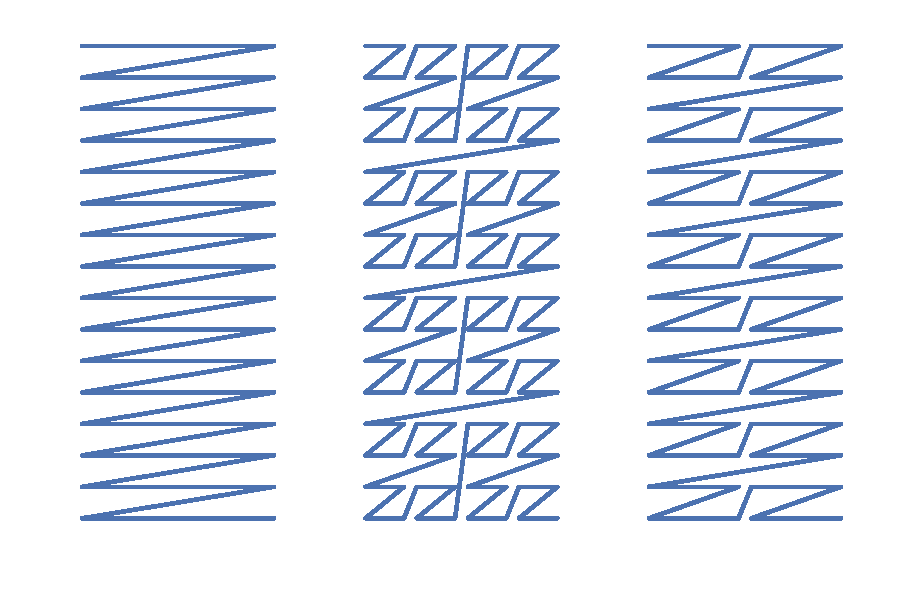
\includegraphics[width=\textwidth]{layouts.pdf}
	\caption{\label{fig:layouts} The different memory layouts described. The blue lines illustrate the order in which the cells in the X-Y-plane of the grid are stored in memory. The lowest memory index always starts at the top-left corner. Left: Row-major indexing. Middle: Normal z-order curve. Right: Widened z-order curve.}
\end{figure}

Z-order curves\cite{wiki:z-curves} represent a more realistic unstructured scenario. Some variation of this layout might be used to represent a true unstructured grid with some irregularities. The aim of Z-order curves is to give most cells with close X-, Y- and Z-coordinates close indices. Locality is achieved by \emph{intertwining} the bits of the X- and Y-components of a coordinate, starting with the X-coordinate at the least-significant bit. The middle graph in figure \ref{fig:layouts} shows a Z-order curve. Observe how the blue line representing the order of memory indices seldom makes large jumps, meaning points that are close in physical space remain close in memory. Compared to the row-major layout (left in that figure), this is a big improvement in locality.

Consider a two-dimensional coordinate, wherein both components are given as a bit string of even length $n$ as:
$$p=\begin{pmatrix}p_x & p_y\end{pmatrix}^\top=\begin{pmatrix}\left\langle p_x^{(n)} p_x^{(n-1)} \cdots p_x^{(2)} p_x^{(1)} \right\rangle & \left\langle p_y^{(n)} p_y^{(n-1)} \cdots p_y^{(2)} p_y^{(1)} \right\rangle\end{pmatrix}^\top$$
The index in Z-order curve ordering is then given by:
\begin{gather}
	i = \left\langle p_y^{(n)} p_x^{(n)} p_y^{(n-1)} p_y^{(n-1)} \cdots p_y^{(2)} p_x^{(2)} p_y^{(1)} p_x^{(1)}\right\rangle
\end{gather}

In this thesis, we have implemented a memory layout wich uses a modified Z-curve layout in the X-Y-plane. To make use of CUDA's vector instructions, which can consume up to 32 bytes of consecutive memory at once when properly aligned, the Z-curve implemented is a stretched out variant. The last five bits are \emph{not} intertwined. To ensure the indices are dense, the cells are then ordered by the number obtained due to this intertwining way and are indexed in a consecutive manner from lowest to highest intertwined number.

Using this, we get repeated lines of 32 cells which share their relative neighborship offsets with other such lines; this allows better coalesced accesses. Using a width of 32 ensures that coalescing is possible even for one-byte data types; when using four- or eight-byte floating point types, the width could be reduced. Despite this optimization, neighborship offsets are more varied with this layout than for the row-major layout, rendering both compression and coalescing less efficient.

Using a truly arbitrary, randomized memory layout was also considered, but not pursued further after initial tests. In grids with a randomized layout, cache locality was completely destroyed, leading to runtimes around eight times the row-major or z-curve variants. For example, the \emph{Laplace-of-Laplace} stencil described in section \ref{sec:results} completed in around $814 \mu s$ for a row-major layout, whereas it took $6999 \mu s$ in a completely random layout in otherwise identical conditions. However, such a completely random memory layout is highly unrealistic. Even in real unstructured meteorology applications, large portions of the grid would remain regular. Unstructuredness only occurs in boundary areas, e.g. between areas of different resolutions. Evaluating the performance implications of a completely random layout provide little value to the implementation of meteorological stencils and possible optimizations would be very limited.


\section{Representing Multiple Fields} \label{sec:representing-multiple-fields}

Two of the three benchmarked stencils and most real-world applications perform calculations that require more than one input value per cell in the grid. There are two obvious approaches to storing multiple \emph{fields} for both regular and unstructured grids, \emph{array-of-structs} and \emph{struct-of-arrays}.

\paragraph{Array of Structs}
In the array-of-structs memory layout, all fields for one cell are stored together, before any values for the next cell. This means that accesses to different fields of the same cell have good memory locality, whereas accessing the same field of different cells requires larger strides.

\paragraph{Struct of Arrays}
In the struct-of-arrays layout, there are $k$ arrays for $k$ fields. This is conceptually the same as having $k$ different one-field grids. Different fields of the same cell are stored in seperate arrays and are thus seperated by (at least) the size of one array. This approach requires additional care to keep the indices for cells synchronized across all arrays; deleting or adding a cell requires access to all $k$ arrays.

The struct-of-arrays approach is highly beneficial to most GPU stencil implementations because of coalescing. When a stencil is implemented such that each thread is responsible for the calculation of one output value, all threads will most likely try to access the same field on different cells concurrently. In the struct-of-array layout, these accesses are able to coalesce (if the cells appear consecutively in memory).  Because of this, we have implemented all our benchmarks in this fashion, i.e. as multiple one-field grids. To verify the claim that array-of-structs is slowr than struct-of-arrays, we have implemented both variants for the \emph{fast waves} benchmark, see table \ref{tab:array-of-structs}.

\begin{table}
	\begin{tabular}{l c c}
		\textbf{Benchmark} & \textbf{Run Time} & \textbf{Load Efficiency} \\
		\hline
		Array of Structs & $8282 \mu s$ & $25.73\%$\\
		Struct of Arrays & $2546 \mu s$ & $99.39\%$
	\end{tabular}
	\caption{\label{tab:array-of-structs} Comparison of run times and global load efficiency (ratio of requested loads to performed loads, where bad coalescing leads to more loads being performed than needed) for the fast waves benchmark with domain size $512\times 512\times 64$ and block size of $128\times 1\times 2$.}
\end{table}

However, in the struct-of-arrays approach, cache locality might suffer from the large strides between the fields of a cell. It might be desirable to also load the other fields of a cell into the cache when one field of that cell is accessed. In this approach, however, only identical fields from other cells are close and thus loaded in the cache. A compromise that seeks to combine both the caching advantages of array-of-structs and the coalescing of struct-of-arrays is the \emph{array-of-structs-of-arrays} approach, which stores one array, which for each warp-sized block of cells contains a struct of warp-sized arrays for each field. We have not implemented this.

\chapter{Grid Access Strategies} \label{sec:optimizations}

In a stencil, computation of the output value of one cell requires access to a neighborhood of cells. Accessing a cell's neighbor's value entails determining the coordinates of the desired neighbor and subsequently calculating the memory index of those coordinates. For structured grids, both of those tasks involve only arithmetic (as described in the indexing section). For unstructured grids, neighbor access in the X-Y-plane requires an additional memory lookup. This is not necessary for neighbors in the Z-direction, as the grid is regular in this direction.

In this chapter, we describe how stencils can obtain the index of required neighbors and access the grid in optimized ways.

\section{Naive Grid Access and Index Variables}

\subsection{Naive} In the \emph{naive} grid access approach, one thread is mapped to each output cell (total of $d_x*d_y*d_z$ threads). The indexing and neighborship calculations (including the memory lookup required for unstructured grids) are (re-)performed each time a cell's value is accessed in a stencil.  One inefficiency of this approach is that most stencils require the same neighboring cells multiple times in different parts of their calculations. Even though the structure of the grid does not change, the indexing calculations are redone in the naive approach on every neighbor access.

\subsection{Index Variables} The \emph{index variables} approach (\emph{idxvar} for short) addresses issue described for the \emph{naive} approach. There is also one thread per output cell. In this variant, in the first phase of the kernel, all required cell's indices are calculated and stored in variables. These index variables are then used whenever a neighboring cell's value needs to be accessed. This ensures that indexing/neighborship calculations are only performed once, even if the same cell is accessed multiple times within one thread. The additional index variables potentially increase the register usage of the kernel, but they reduce the number of expensive memory lookups into the neighborship table if the same neighbors are re-accessed within the same kernel.

\section{Optimizations Making Use of the Z-Regularity}

\subsection{Index Variables + Shared Memory} In this approach (\emph{shared} for short), the stencil is implemented such that there is one thread per output cell (as in \emph{naive} and \emph{idxvar}). However, not all threads perform the neighbor index lookups. Instead, for each cell in the X-Y-plane, designated ``leader'' threads in each block perform the index calculation/lookup of all required neighboring cells at the $Z=0$ level. The designated threads store the result of that computation/lookup in shared memory. If the Z-index modulo the Z-block-size is zero, a thread is a designated lookup-thread. After the indices of the neighboring cells at the lowest Z-level are determined and stored in shared memory, all threads in the block synchronize. All threads then access shared memory to obtain the required indices. They add the appropriate constant Z-stride to them to obtain the index of the neighbors at their Z-level. Using this approach, the regularity of the grid in the Z-dimension is exploited in order to only perform one global memory lookup per block for the neighborship information. The shared memory lookups are cheaper than lookups in global memory, but synchronization adds some overhead. For this approach to be effective, the block size in the Z dimension needs to be large enough.

\subsubsection{Bank Conflicts}

As mentioned in section \ref{sec:bank-conflicts}, bank conflicts occur in the Volta architecture when two threads try accessing addresses that are equal modulo $32$. Bank conflicts have to be avoided in order to make use of the full performance of shared memory.

A thread in the \emph{shared} access strategy stores or reads multiple shared memory slots (one for each neighbor). Assume we store neighborship information of each cell contiguously in shared memory. If the total number of required neighbors is very unfortunate, for example $8$ neighbors per cell (equals an array of $32$ bytes), then all threads end up (trying to) access the same memory bank simultaneously in the index lookup phase. This happens because the length of the neighborship array happens to align all top neighbors of cells into one bank, all left neighbors into another bank, etc. In the index lookup phase, all threads then attempt to load their top (left, ...) neighbor pointer at the same time.

In the \emph{shared} access strategy we address this problem by adding padding to the shared memory storage of neighbors. Thus, neighbors are not stored contiguously, but have gaps in between them. The padding is chosen as the smallest value that is coprime with $32$. This guarantees the least possible number of bank conflicts in this scenario; pointers to the same type of neighbor are spread out evenly across banks for different cells. In other words, all top neighbors are spread evenly across banks, all left neighbors are spread evenly across banks (but may coincide banks with top neighbors, because those are not accessed at the same time instant), etc.

\subsubsection{Warp Broadcasting}

\begin{table}
    \begin{tabular}{l l l l}
        \hline
        \textbf{Block size} & \textbf{Variant} & \textbf{Runtime} \\
        \hline
        \hline
        $128\times 1 \times 8$ & Shared memory        & $\mathbf{684 \mu s}$ \\
                               & Warp broadcasting & $737 \mu s$ \\
        \hline
        $32\times 1\times 8$ & Shared memory & $\mathbf{675 \mu s}$ \\
                             & Warp broadcasting & $693 \mu s$ \\
        \hline
        $1\times 1\times 32$ & Shared memory & $13654 \mu s$ \\
                             & Warp broadcasting & $\mathbf{12711 \mu s}$ \\
        \hline
    \end{tabular}
    \caption{\label{tab:warp-broadcasting}Median runtimes (20 runs) for the Laplace-of-Laplace benchmark (z-curves memory layout, pointer chasing, uncompressed) for three select block sizes. We observe that warp broadcasting is only faster than shared memory in the last block size configuration, which is the slowest overall. We therefore did not further investigate the use of warp broadcasting.}
\end{table}
% ./gridbenchmark --no-verify --size 512x512x64 --threads 128x1x8 32x1x1 32x1x8 8x1x32 1x1x32 laplap-unstr-idxvar-shared -z laplap-unstr-idxvar-warp-shared -z 
% Benchmark                           , Precision, Domain size,,, Blocks     ,,, Threads    ,,, Kernel-only execution time                
%                                    ,          ,   X,   Y,   Z,   X,   Y,   Z,   X,   Y,   Z,   Average,    Median,   Minimum,   Maximum
% laplap-unstr-idxvar-shared-z-curves-4,    double, 512, 512,  64,   4, 508,   8, 128,   1,   8,    685276,    684060,    675086,    696476
% laplap-unstr-idxvar-shared-z-curves-4,    double, 512, 512,  64,  16, 508,  64,  32,   1,   1,   1038436,   1037644,   1027729,   1046049
% laplap-unstr-idxvar-shared-z-curves-4,    double, 512, 512,  64,  16, 508,   8,  32,   1,   8,    673723,    674726,    654446,    691286
% laplap-unstr-idxvar-shared-z-curves-4,    double, 512, 512,  64,  64, 508,   2,   8,   1,  32,   2114038,   2114163,   2111828,   2116009
% laplap-unstr-idxvar-shared-z-curves-4,    double, 512, 512,  64, 508, 508,   2,   1,   1,  32,  13804636,  13653834,  13220255,  14550507
% laplap-unstr-idxvar-warp-shared-z-curves-4,    double, 512, 512,  64,   4, 508,   8, 128,   1,   8,    737049,    737926,    725546,    742856
% laplap-unstr-idxvar-warp-shared-z-curves-4,    double, 512, 512,  64,  16, 508,  64,  32,   1,   1,   1010478,   1010224,   1004369,   1017049
% laplap-unstr-idxvar-warp-shared-z-curves-4,    double, 512, 512,  64,  16, 508,   8,  32,   1,   8,    695580,    693476,    683075,    766056
% laplap-unstr-idxvar-warp-shared-z-curves-4,    double, 512, 512,  64,  64, 508,   2,   8,   1,  32,   1860175,   1860061,   1856796,   1863697
% laplap-unstr-idxvar-warp-shared-z-curves-4,    double, 512, 512,  64, 508, 508,   2,   1,   1,  32,  12711574,  12712320,  12702761,  12722870

Loads and stores to shared memory produce some overhead. A more lightweight alternative provided by the Cuda architecture are so-called \emph{warp-level primitives}. Those allow threads that are \emph{within the same warp} to exchange data more efficiently -- in a direct register-to-register fashion.

We briefly experimented with a variant of \emph{shared} strategy, using warp broadcasting instead of shared memory. In this variant, all threads in the first lane (first thread of each warp) are the designated leader threads that do the actual neighbor lookup. Other threads in the same warp receive the leader thread's pointer by use of the \texttt{\_\_shfl\_sync()} method.

While the actual warp broadcasting is more lightweight than shared memory, it is also more limited: only threads within the same warp can exchange data. This sets restrictions on the kernel launch configuration; the threads in a block have to be allocated such that cells across different Z-levels fall within the same warp (otherwise no neighbor pointer sharing can take place). To make use of warp broadcasting, some additional calculations also need to be made (determining the lane ID, masks of active threads). For those reasons, warp broadcasting appeared to be slightly slower than the shared memory access variants in most realistic scenarios. In launch configurations with many threads in the X- or Y-dimension, warp broadcasting even was considerably slower (due to no sharing being possible within warp limits anymore). However, in launch configurations with many threads in the Z-dimension, warp broadcasting slightly outperformed shared memory. These launch configurations are rather slow overall (compared to other block sizes), though, and are therefore not very useful.

See table \ref{tab:warp-broadcasting} for a comparison of the warp broadcasting approach to using shared memory on an exemplary benchmark.

\subsection{Index Variables + Z-loop} In this approach (\emph{z-loop} for short), there are only $d_x\times d_y$ threads, i.e. only one thread per stack of cells in the X-Y-plane. Each thread calculates the results for all cells with equal X- and Y-coordinates in a loop over all Z. The indices of all required cells at the $z=0$ level are stored in \emph{index variables} before the start of the loop. The regularity of the grid in Z-direction enables us to update the index variables in each iteration of the loop by simply adding a Z-stride. There is no memory lookup into the neighborship table inside the loop. Thus, even in the unstructured grid case, memory lookups are only necessary once before the loop. This comes at the cost of possibly reduced occupancy, however, as there are fewer threads.

\subsection{Index Variables + Sliced Z-loop} This variant addresses the issue of low occupancy in the above approach. It is practically identical to it, but splits the Z-loop up in smaller chunks. There are $d_x\times d_y\times \frac{d_z}{m}$ threads, where $m$ is the number of output cells in the Z-direction a single thread should calculate. In the following benchmarks, we used $m=8$.

%\paragraph{Loop Unrolling}
% TODO mention effects of loop unrolling in the latter two variants


\chapter{Benchmark Results}    \label{sec:results}

In this section, we seek to determine the overhead that indirect addressing imposes on unstructured grids compared to regular grid runtimes, and assess the effectiveness of our optimized approaches. We do this by implementing three real-world stencils, called \emph{Laplace-of-Laplace (laplap)}, \emph{horizontal diffusion (hdiff)}, and \emph{fastwaves}, using our previously described methods for grid access and grid storage (see sections \ref{sec:optimizations} and \ref{sec:grid-implementations}). We use key profiler metrics to better understand what causes the differences in performance.

Real-world stencil applications are applied in a multitude of different scenarios: problem domain sizes, precision requirements and properties of the stencils vary. In combination with the various grid access and grid storage methods we described, this leaves a large number of combinations to be tested. In our benchmarks, we assessed the performance impact of the following properties:

\begin{itemize}
    \item 
        Input/output conditions 
        \begin{itemize}
            \item Domain size (size of the input and output grids)
            \item Required precision (single or double floating-point number precision)
        \end{itemize}
    \item
        Stencil properties, such as the \emph{depth and number of neighbor dependencies}, the \emph{number of input and output fields} (number of different values stored in a cell) and the \emph{arithmetic intensity}
    \item
        \emph{Kernel launch configuration:} number of threads, blocks, and bytes of shared memory
	\item Implementation of stencil, i.e. the used \emph{grid access scheme}
    \item
        Grid storage implementation properties
        \begin{itemize}
            \item Memory layout and potential regular patterns in grid structure
            \item 
                Memory layout of neighborship storage
                \begin{itemize}
                    \item Depth of stored neighbor pointers (pointer \emph{chasing} vs. \emph{non-chasing})
                    \item Compression of neighborship table
                \end{itemize}
        \end{itemize}

\end{itemize}

\section{Setup and Benchmarked Stencils}\label{sec:benchmark-setup}

The three benchmarked stencils represent real-world use cases in meteorology. Table \ref{tab:benchmarked-stencils} details the values of the main stencil characteristics (those listed in the second main bullet point above). Note the increasing complexity and number of fields required from the \emph{laplap} to the \emph{fastwaves} stencil. Also note that the \emph{fastwaves} stencil, otherwise the most complex, does not require access to neighbors-of-neighbors.

\begin{table}
	\makebox[\textwidth][c]{                                     
		\begin{tabular}{m{4cm} m{1.25cm} m{1.25cm} m{1.25cm} m{1.25cm} m{4cm}}
		    \textbf{Stencil}  &  \multicolumn{3}{c}{\textbf{Neighborhood}}  &  \textbf{Fields}  &  \textbf{Arithmetic Intensity} \\
		    \cline{2-4}
		    &  \textbf{X}  &  \textbf{Y}  &  \textbf{Z}  & \\
		    \hline
			\hline
		    \raggedright Laplace-of-Laplace \emph{(laplap)}  &  (-2, 2)  &  (-2, 2)  &  0  &  1  & {\raggedright Add., Mult., Sub.} \\
			\hline
		    \raggedright Horizontal Diffusion \emph{(hdiff)}  &  (-2, 2)  &  (-2, 2)  &  0  &  2  &  {\raggedright Add., Mult., Sub., Branches} \\
			\hline
		    \raggedright \emph{Fastwaves}  &  (0, 1)  &  (0, 1)  &  (-1, 1)  &  9  & {\raggedright Add., Mult., Sub., Div., Branches} \\
		    \hline
		\end{tabular}
	}
	\caption{\label{tab:benchmarked-stencils}Stencil characteristics. The neighborhood is given as an interval around the coordinates of a cell, i.e. $(-2, 2)$ means neighbors-of-neighbors are required for the stencil output calculation. The stencils are listed by their regular grid runtime in ascending order. Note that the \emph{fastwaves} stencil is the only stencil with dependencies in the Z-dimension, has the highest arithmetic intensity, and accesses the biggest number of fields.}
\end{table}

The calculations performed by the stencils are defined in terms of a regular grid. All three stencils require neighborships as in regular grids (top, left, bottom, right, front, back). To measure the cost of using an unstructured grid, we represent the same regular grid in an unstructured fashion, using two memory layouts, \emph{row-major} and \emph{z-order-curves} (see section \ref{sec:emulating}). This can be thought of as \emph{emulating} an unstructured grid. Even if the grid structure is entirely regular, we store and access it in the same fashion as we would for a truly unstructured grid in the unstructured benchmarks. Retaining regularity even in the unstructured representation is required to maintain comparability of the results of the unstructured variants with the regular variants. We note that this approach to benchmarking might fail to capture some effects of real unstructured grids with actual irregularities.

For all stencils, we created several variants; for each of the grid access optimizations described in section \ref{sec:optimizations} we implemented a separate CUDA kernel. During the implementation process, the results of each of those variants are verified against an unoptimized reference implementation of the stencil running on the CPU to assure the correctness of the results. In all variants, the implementation of the actual output calculations (as per stencil definition) remains completely unchanged. Only the portions of code responsible for index calculations/lookups (for neighborship access) are swapped out. This is achieved by using \emph{C preprocessor macro definitions} in all places where indexing or neighborship access is required. The macro definitions are then redefined in each variant to either use direct or indirect addressing for the regular and unstructured grids, respectively (with further variations for non-chasing/chasing and compressed/uncompressed neighborship tables).

The stencils were benchmarked on an \emph{Nvidia Tesla V100} GPU. This GPU implements the \emph{Volta} architecture by Nvidia with compute capability $7.0$. The reported run times are the median of 20 timed kernel runs. Before the first one of the timed kernel runs, an untimed \emph{warm-up run} is performed (see the last paragraph section \ref{sec:arguing} for the reasoning behind this). The GPU is reset using an API call to \texttt{cudaDeviceReset()} between each run to flush caches and to free device memory from previous runs. The grid values and neighborship relations (for unstructured grids) are stored in unified global memory and are pre-transferred to the GPU and back to the host (\texttt{cudaMemPrefetchAsync()}) before respectively after the kernels are run. Memory transfer from host to device and back is, therefore, \emph{not} part of the reported run times.

\section{Overview of Results}

\begin{figure}
    % >>> fas=u.groupmin(df[(df["size-z"]==64)&df["z-curves"]], by=u.col.problem+u.col.access+u.col.storage)
    % >>> fas=u.add_colors_markers(fas, color="variant")
    % >>> reg=u.groupmin(df[(df["size-z"]==64)&~df["unstructured"]], by=u.col.problem)
    % >>> reg["variant"]="regular"
    % >>> reg["color"]="black"
    % >>> x=pd.concat([fas,reg])
    % >>> u.barplot(x[x["stencil"]=="fastwaves"], grp=u.col.storage+["unstructured"], cat=u.col.access, cat_pretty=["variant"], grp_pretty=["no-chase", "comp"])
    % <matplotlib.axes._subplots.AxesSubplot object at 0x124582ed0>
    % >>> plt.ylabel("Median runtime [μs]")
    % Text(0, 0.5, 'Median runtime [μs]')
    % >>> fig=u.plotdone(legend=2)
    % >>> fig.set_size_inches(6,3)
    % >>> u.plotsave("report/img/overview-fastwaves.pdf", fig)
	\begin{center}
	    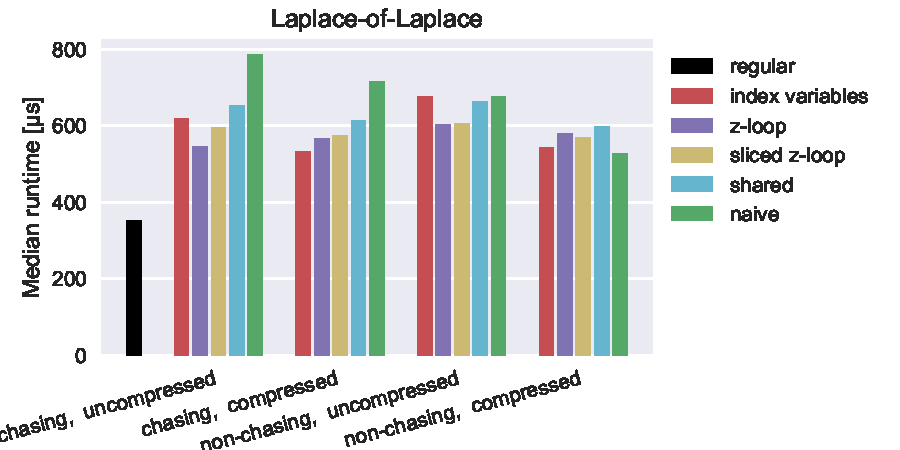
\includegraphics[scale=0.75]{overview-laplap.pdf}
    
	    \vspace{0.5cm}
    
	    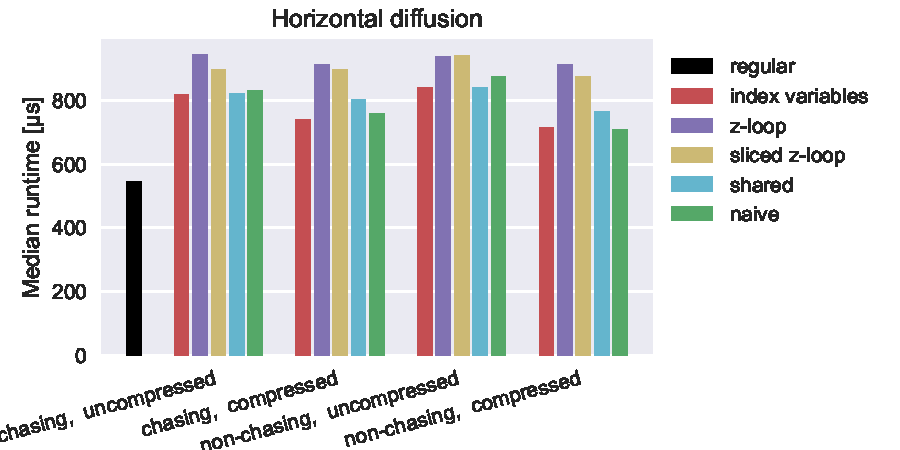
\includegraphics[scale=0.75]{overview-hdiff.pdf}
    
	    \vspace{0.5cm}
    
	    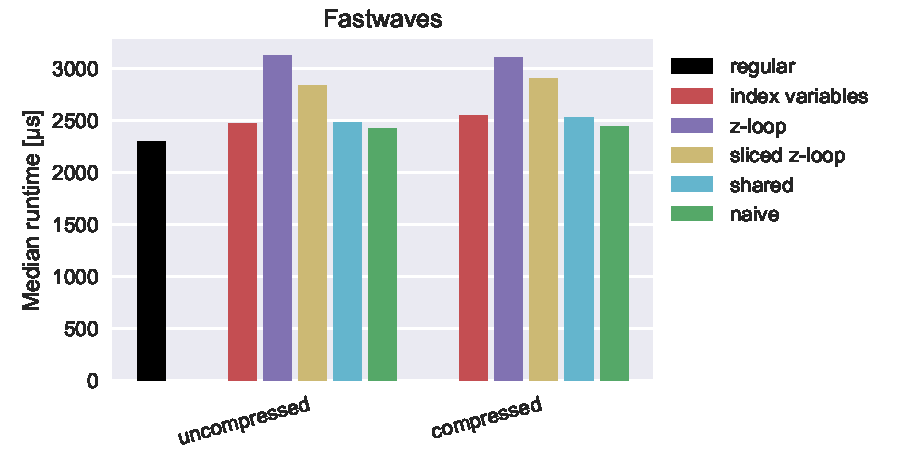
\includegraphics[scale=0.75]{overview-fastwaves.pdf}
		
    \end{center}
    \caption{\label{fig:storage-access} Overview of runtimes for all tested stencil implementations. The various grid access strategies implemented are represented as categories (colors of the bars), while the used data structures for the neighborship table (grid storage strategy) are shown as groups of bars on the X-axis. We report the median value across 20 runs, using the fastest respective launch configuration for each bar. The grid size is $512\times 512\times 64$ and the \emph{z-curves} memory layout is used for the unstructured grids in this example. The input and output values are double-precision floating-point numbers.}
\end{figure}

\begin{table}
	\begin{center}
    \begin{tabular}{l c c l c r} % c c}        
        \multicolumn{6}{c}{\textbf{Laplace-of-Laplace Stencil}} \\
        \hline
        \hline
        %& & & & \multicolumn{2}{c}{$512\times 512\times 64$ Grid} & \multicolumn{2}{c}{$128\times 128\times 64$ Grid} \\
        %\cline{5-6} %\cline{7-8} 
        Storage & (1) & (2) & Access Strategy  & Runtime & Slowdown \\ %& Runtime & Slowdown \\
        \hline 
        \multicolumn{3}{l}{regular grid baseline} & index variables & $353 \mu s$ & -\\
        \hline
         row-major & \checkmark & \checkmark & index variables &  $\mathbf{512 \mu s}$ & $\mathbf{45 \%}$ \\
         row-major & - & \checkmark & index variables & $515 \mu s$ & $46 \%$ \\
         row-major & \checkmark & - & sliced z-loop & $582 \mu s$ & $65\%$ \\
         row-major & - & - & sliced z-loop & $608 \mu s$ & $72 \%$ \\
        \hline
         z-curves & - & \checkmark & naive & $\mathbf{528 \mu s}$ & $\mathbf{50 \%}$ \\
         z-curves & \checkmark & \checkmark & index variables & $532 \mu s$ & $51 \%$ \\
         z-curves & \checkmark & - &  z-loop & $546\mu s$ & $55 \%$ \\
         z-curves & - & - & z-loop & $603 \mu s$ & $71 \%$ \\
        
        \hline
        \hline \\
        \multicolumn{6}{c}{\textbf{Horizontal Diffusion Stencil}} \\
        \hline
        \hline
        Storage & (1) & (2) & Access Strategy  & Runtime & Slowdown \\
        \hline
        \multicolumn{3}{l}{regular grid baseline} & index variables & $546 \mu s$ & - \\
        \hline
          row-major & - & \checkmark & naive & $\mathbf{683 \mu s}$ & $\mathbf{25 \%}$ \\
        
         row-major & \checkmark & \checkmark & index variables & $731 \mu s$ & $34 \%$ \\
        
         row-major & \checkmark & - & index variables & $804\mu s$ & $47\%$ \\
         &   & &  shared (tie) & $804\mu s$ & $47\%$ \\
         row-major & - & - & naive & $845 \mu s$ & $55 \%$ \\
        \hline
         z-curves & - & \checkmark & naive & $\mathbf{710 \mu s}$ & $\mathbf{30 \%}$ \\
         z-curves & \checkmark & \checkmark & index variables & $741 \mu s$ & $36 \%$ \\
         z-curves & \checkmark & - & index variables & $820\mu s$ &  $50 \%$ \\
         z-curves & - & - & shared & $841 \mu s$ & $54 \%$ \\
        
        \hline
        \hline\\
        \multicolumn{6}{c}{\textbf{Fastwaves Stencil}}\\
        \hline
        \hline
        Storage & (1) & (2) & Access Strategy  & Runtime & Slowdown \\
        \hline
        \multicolumn{3}{l}{regular grid baseline} & naive & $2298 \mu s$ & - \\
        \hline
        row-major & & - & naive & $\mathbf{2400\mu s}$ & $\mathbf{4.4 \%}$ \\
        row-major & & \checkmark & naive & $2433\mu s$ & $5.9 \%$ \\
        \hline
        z-curves & & - & naive & $\mathbf{2426\mu s}$ & $\mathbf{5.6 \%}$ \\
        z-curves & & \checkmark & naive & $2438\mu s$ & $6.1 \%$ \\
        \hline\hline
    \end{tabular}
	\end{center}
    \begin{enumerate}[label=(\arabic*)]
        \item \textbf{Pointer Chasing?} (A checkmark means that only directly adjacent neighbors are stored and pointer chasing occurs for neighbor-of-neighbor access. No checkmark means neighbors-of-neighbors are explicitly stored in the neighborship tables.)
        \item \textbf{Compressed?} (A checkmark means the neighborship table was compressed by having all cells with identical relative neighbor offsets share their entries. This requires an additional lookup.)
    \end{enumerate}
    \caption{\label{tab:overview} Fastest access strategy for all grid storage options. \emph{Z-curves} and \emph{row-major} refer to the memory layout of the \emph{values} of the grid, whereas \emph{chasing/non-chasing} and \emph{compressed/uncompressed} are properties of the neighborship table. The runtimes are the median of 20 runs using the fastest respective launch configuration per benchmark. The slowdown is relative to the fastest regular grid implementation. The stencils were executed on a $512\times 512\times 64$-sized grid of double-precision floating-point numbers.}
\end{table}

Overall, we observed slowdowns around $1.5x$, $1.3x$ and $1.05x$ compared to fastest regular grid performance for the \emph{laplap}, \emph{hdiff} and \emph{fastwaves} stencils, respectively. Figure \ref{fig:storage-access} shows an overview of the overhead for all tested combinations of storage and access strategy on a large grid of size $512\times 512\times 64$. Table \ref{tab:overview} lists the fastest access strategy, the runtimes and the overheads for the three stencils in all possible storage configurations. For different domain sizes, see section \ref{sec:res-size}. We chose to display the results for a \emph{z-curve} layout, but results for the \emph{row-major} benchmarks are similar. The fastest launch configuration is plotted for each bar; for a more detailed analysis of what block sizes are beneficial to the different access strategies, see section \ref{sec:res-blocksize}. A more in-depth analysis of the different storage and access strategies is given in sections \ref{sec:res-storage} and \ref{sec:res-access} respectively.
\section{Optimal Block Size} \label{sec:res-blocksize}

% TODO make concrete suggestions for optimal block size (table maybe?)

% \begin{table}
%     \begin{tabular}{l p{2.35cm} p{2.35cm} p{2.35cm} p{2.35cm}}
%         \hline
%         Access & {\raggedright chasing, uncompressed} & {\raggedright non-chasing, uncompressed} & {\raggedright chasing, compressed} & {\raggedright non-chasing, compressed} \\
%         \hline
%         \hline
%         hdiff & & & & \\
%         \emph{naive} & $32\times 1\times 8$ & $64\times 1\times 8$ & $256\times 1\times 1$ & $128\times 1\times 2$ \\
%         \emph{idxvar} & $64\times 1\times 8$ & $32\times 1\times 16$ & $128\times 1\times 2$ & $64\times 1\times 2$ \\
%     \end{tabular}
% \end{table}

One of the main determining factors for the performance of a kernel is the launch configuration, which includes grid size (number of blocks) and block size (number of threads, described in section \ref{sec:hardware}). As we implemented and evaluated our grid storage and grid access strategies, we consistently ran our benchmarks across a large range of launch configurations. In the previous sections, we reported best-case runtimes using the respective optimal launch configuration. This optimal configuration varies heavily depending on the implementation, as we will detail in this section.

Cuda provides the option to specify block sizes in three dimensions, providing each thread with an X-, Y- and Z-index. In our benchmarks, we have tested all possible combinations of block sizes in steps of powers of two from $32$ up to $512$. In order to cover the entire problem domain (which remains constant in size), a decrease in the number of threads is always accompanied by an increase in the number of blocks (grid size) and vice versa. Owing to the way we map thread indices onto memory indices (X thread index maps onto memory index directly), thread sizes in the X-dimension of less than $32$ are highly inefficient, as they lead to non-coalescing memory accesses. The X-dimension of the benchmarked block sizes is therefore always at least $32$.

\subsection{Overview}

\begin{figure}
	\begin{center}
    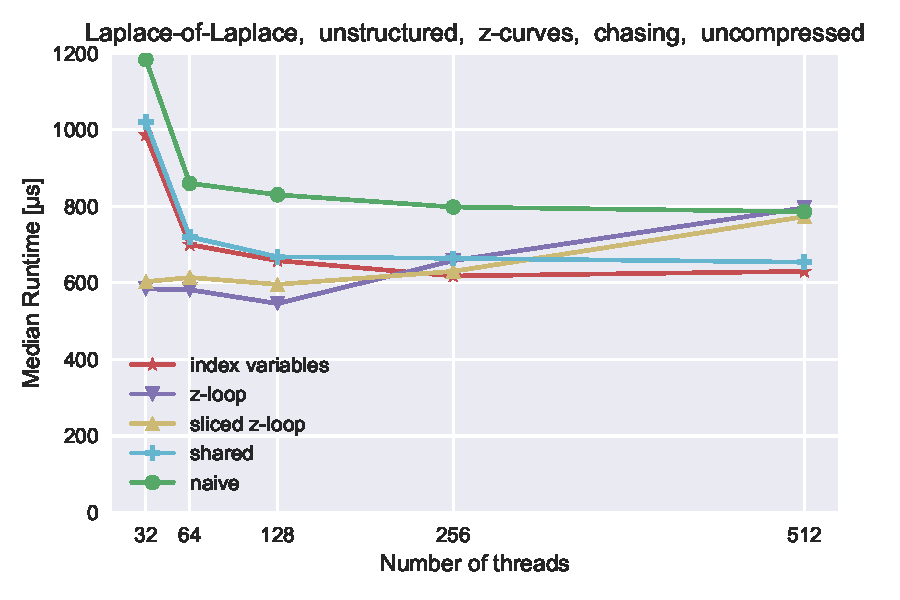
\includegraphics[scale=0.75]{threads-total-laplap.pdf}
	\end{center}
    \caption{\label{fig:blocksizes-overview} Impact of total block size (product of X-, Y- and Z-blocksize) on the runtime for different implementations of the \emph{laplap} stencil on a $512\times 512\times 64$-sized grid (\emph{z-curves} memory layout with \emph{double} precision, \emph{chasing} and \emph{uncompressed} neighborship table). The low-occupancy \emph{z-loop} and \emph{z-loop-sliced} access strategies do not profit from a larger number of threads, contrary to the other variants. Results for other stencils and variants are of similar shape.}
% >>> u.lineplot(df[(df["size-z"]==64)&(df["stencil"]=="laplap")&df["z-curves"]&~df["no-chase"]&~df["comp"]], x="threads-prod", y="median")
% >>> plt.ylabel("Median Runtime [µs]")
% Text(0, 0.5, 'Median Runtime [µs]')
% >>> plt.ylim(0, 1200)
% (0, 1200)
% >>> plt.grid("both")
% >>> fig=u.plotdone(legend=0)
% >>> u.plotsave("report/img/threads-total-laplap.pdf", fig)
\end{figure}

The optimal \emph{total number} of threads depends mostly on the grid access implementation employed. In general, the same patterns can be observed for all three tested stencils and all tested grid memory storage implementations: When using the \emph{naive}, \emph{idxvar} or \emph{shared} grid access strategies, it is best to have a high number of threads in total ($256-512$). The \emph{z-loop} and \emph{z-loop-sliced} thrive on a lower number of threads due to occupancy concerns. An exemplary overview of the runtimes as a function of total block size is given in figure \ref{fig:blocksizes-overview}.

\begin{figure}
	\begin{center}
    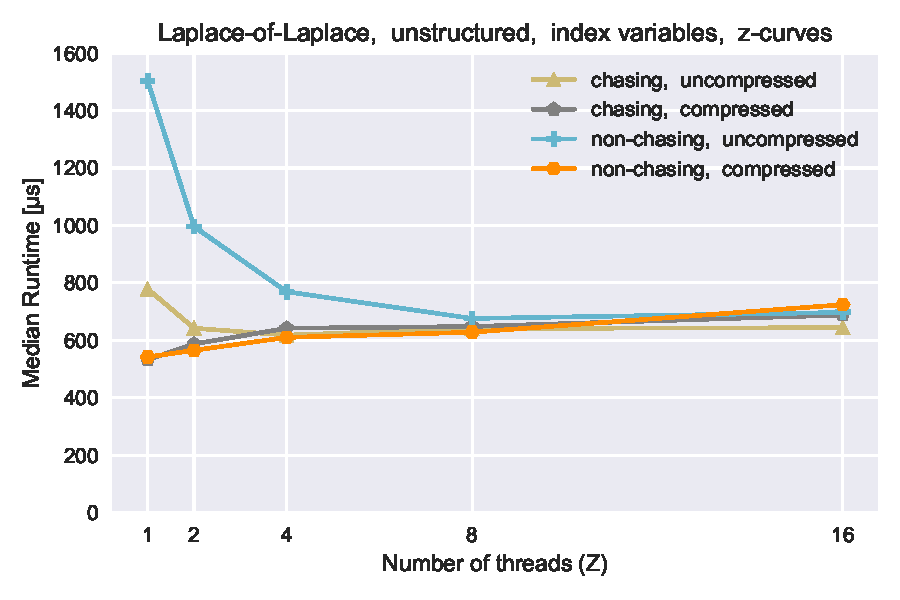
\includegraphics[scale=0.75]{threads-z-storages.pdf}
% >>> u.lineplot(df[(df["size-z"]==64)&(df["stencil"]=="laplap")&df["z-curves"]&df["unstructured"]&(df["variant"]=="idxvar")],by=["no-chase", "comp"], x="threads-z", y="median")
% >>> plt.ylabel("Median Runtime [µs]")
% Text(0, 0.5, 'Median Runtime [µs]')
% >>> plt.grid("both")
% >>> plt.ylim(0, 1600)
% (0, 1600)
% >>> fig=u.plotdone(legend=0)
% >>> u.plotsave("report/img/threads-z-storages.pdf", fig)
	\end{center}
    \caption{\label{fig:blocksizes-z}Fastest runtimes of all configurations for fixed numbers of threads in the Z-dimension (other dimensions free) for the \emph{laplap} stencil on a $512\times 512\times 64$-sized domain (\emph{row-major} memory layout with \emph{double} precision) for \emph{compressed} and \emph{uncompressed} variants, with and without pointer \emph{chasing}. Note how the Z-regularity of the grid makes it advantageous to have a larger number of threads in the Z-dimension, as this leads to caching of neighborship table entries, but only if the neighborship table is \emph{uncompressed}.}
\end{figure}

The best \emph{shape} of the block size vector changes with the used grid storage strategy. Using \emph{uncompressed} neighborship tables, it is best for the \emph{naive}, \emph{idxvar} and \emph{shared} access strategies to have $32$ or $64$ threads in X-dimension and the rest in Z-dimension. Those implementations profit of more Z-threads because of the regularity of the grid in the Z-dimension. The \emph{non-chasing} variants profit even more of additional threads in the Z-dimension. This is because, in non-chasing variants, more neighborships are stored in the table; cache entries are thus evicted faster if many different X- and Y-coordinates are accessed. In \emph{compressed} neighborship tables, on the other hand, additional threads in the Z-dimension are of no use to any of the access strategies -- the greatly reduced number of neighborship table entries after compression remains in cache independent of the Z-block-size. See figure \ref{fig:blocksizes-z} for a comparison of how changes in the Z-dimension of the block size vector translate to runtime changes. Whether the grid is stored as \emph{row-major} or using \emph{z-order} curves does not strongly impact the required block sizes.

\subsection{Optimal Block Sizes per Access Strategy}

In this section, we further elaborate on the optimal block sizes for each access strategy and aim to explain (using profiler metrics) why certain shapes of thread blocks are beneficial.

\subsubsection{\emph{Naive}, \emph{Idxvar} and \emph{Shared} Grid Access Strategies}

In order to always cover the entire problem domain, the number of blocks $b$ in each dimension in the \emph{naive}, \emph{idxvar} and \emph{shared} grid access strategies is chosen as a function on the problem size $d$ and the chosen number of threads $t$ as follows:
$$b = \begin{pmatrix}\left\lceil\frac{d_x}{t_x}\right\rceil & \left\lceil\frac{d_y}{t_y}\right\rceil & \left\lceil\frac{d_z}{t_z}\right\rceil\end{pmatrix}^\top$$

For the \emph{naive}, \emph{idxvar} and \emph{shared} implementations, a high total number of threads per block is beneficial to performance. For grids using an \emph{uncompressed} neighborship table, increasing the number of threads in the Z-dimension especially improves performance.

\begin{table}
%    \begin{tabular}{l l l l l}
%        Blocksize & \texttt{global\_hit\_rate} & \texttt{tex\_cache\_hit\_rate} & \texttt{l2\_tex\_read\_hit\_rate} & \texttt{l2\_tex\_hit\_rate} \\
%        \hline
%        $32\times 1\times 1$ & $45.42\%$ & $44.39\%$ & $73.86\%$ & $67.69\%$ \\
%        $32\times 1\times 2$ & $58.83\%$ & $57.96\%$ & $76.60\%$ & $68.12\%$ \\
%        $64\times 1\times 2$ & $62.25\%$ & $66.21\%$ & $69.99\%$ & $60.36\%$ \\
%        $64\times 1\times 4$ & $72.33\%$ & $71.72\%$ & $72.77\%$ & $60.81\%$
%    \end{tabular}
	\begin{center}
    \begin{tabular}{l l l p{2cm} p{2cm}}
        \hline
        \textbf{Blocksize} & \textbf{\texttt{tex\_\allowbreak cache\_\allowbreak hit\_\allowbreak rate}} & \textbf{\texttt{l2\_\allowbreak tex\_\allowbreak hit\_\allowbreak rate}} \\
        \hline
        \hline
        $32\times 1\times 1$ & $44.39\%$ & $67.69\%$ \\
        $32\times 1\times 2$ & $57.96\%$ & $68.12\%$ \\
        $64\times 1\times 2$ & $66.21\%$ & $60.36\%$ \\
        $64\times 1\times 4$ & $71.72\%$ & $60.81\%$ \\
        \hline
    \end{tabular}
	\end{center}
    \caption{\label{tab:laplap-blocksize-metrics} Cache hit rates for different block sizes for the \emph{laplap} stencil, implemented using a \emph{idxvar} grid access strategy on a $512\times 512\times 64$-sized domain (\emph{z-curves} memory layout with \emph{double} precision, \emph{chasing} and \emph{uncompressed} neighborship table).}
\end{table}

For the \emph{naive} and \emph{idxvar} strategies (in grids using uncompressed neighborship tables), the advantage of multiple Z-threads can be explained through the regularity of the grid in the Z-dimension. Threads operating on cells with identical X- and Y-coordinates access the neighborship tables at the \emph{same index}. When multiple threads operate on different Z-levels, caching of these shared neighborship table entries becomes very effective. Evidence for this presumed reason for the speedup is given by two facts: One, of all block size combinations tested, the ones with more threads in the Z-dimension perform best. Two, the Nvidia profiler reports higher cache hit rates if the number of threads in Z-dimension is increased. As an example of this for the \emph{idxvar} access strategy, see table \ref{tab:laplap-blocksize-metrics}.

These effects are strongest when using \emph{non-chasing} grid storage. As this type of storage leads to a larger number of entries in the neighborship table, entries may be evicted from the cache more quickly. More threads in the Z-dimension, which access the same neighborship table entries, prevent this by keeping the relevant neighborship table entries ``fresh.''

At the opposite end of the spectrum lie the grids stored using \emph{compressed} neighborship tables. These tables are much smaller, and the same few entries are accessed in almost all threads. Because of this, neighborship table entries remain in cache no matter what the shape of the block size vector is, and additional threads in the Z-dimension bring no benefit. Cache locality for the accessed values is more important here; depending on the used layout for the values (\emph{z-curves} or \emph{row-major}) this means adding additional threads in X (\emph{z-curves}, spatial locality given), or X and Y (\emph{row-major}, adding another thread in Y gives some spatial locality).

By the design of the \emph{shared} access strategy, a speedup is supposed to be attained with a larger number of Z-threads; if there are more threads in Z-dimension within a block, more sharing of neighborship relations through shared memory can take place. These implementations indeed profit from more threads through shared memory in much the same way as \emph{naive} and \emph{idxvar} variants profit from more threads through the cache in the uncompressed grids.

\subsubsection{\emph{Z-loop} and \emph{Z-loop-sliced} Grid Access Strategies}

\begin{table}
	\begin{center}
    \begin{tabular}{l l l p{2.5cm} p{2.5cm}}
        \hline
        \textbf{Variant} & \textbf{Blocksize} & \textbf{Runtime} & \textbf{\texttt{achieved\_\allowbreak occupancy}} & \textbf{\texttt{issue\_\allowbreak slot\_\allowbreak utilization}} \\
        \hline
        \hline
        \emph{idxvar} & $512$ & $783\mu s$ & $85\%$ & $19\%$ \\
        \emph{idxvar} & $128$ & $844\mu s$ & $\mathbf{92\%}$ & $18\%$ \\
        \emph{idxvar} & $32$  & $986\mu s$ & $48\%$ & $16\%$ \\
        \emph{z-loop} & $512$ & $796\mu s$ & $25\%$ & $10\%$\\
        \emph{z-loop} & $128$ & $\mathbf{546\mu s}$ & $42\%$ & $13\%$ \\ 
        \emph{z-loop} & $32$  & $584\mu s$ & $41\%$ & $12\%$ \\
        \hline
    \end{tabular}
	\end{center}
    \caption{\label{tab:laplap-blocksize-occupancy} Runtimes and occupancy metrics of \emph{idxvar} and \emph{z-loop} implementations of the \emph{laplap} stencil on an unstructured grid (size $512\times 512\times 64$, \emph{z-curves} memory layout with \emph{double} precision, \emph{chasing} and \emph{uncompressed} neighborship table) for a selection of block sizes. The following block shapes were used: $512 = 256\times 2\times 1$, $128 = 64\times 2\times 1$ and $32 = 32\times 1 \times 1$. This table highlights the occupancy issues the \emph{z-loop} variant faces with too large block sizes. Note how the occupancy drops with an increased number of threads, and how the runtime increases with it.}
\end{table}

Contrary to the other stencils, the \emph{z-loop} and \emph{z-loop-sliced} grid access strategies suffer from a high total thread count. As both of these strategies require one thread to perform calculations for multiple cells on different Z-levels, the total number of blocks and threads required to cover the entire grid is smaller. On the largest tested grid size ($512\times 512\times 64$), this leads to occupancy issues: As threads stall, there is not enough work that can be scheduled to certain streaming multiprocessors to hide the latency. All threads inside a block are required to be executed on the same SM; having more threads inside a block thus gives fewer blocks that can be scheduled onto stalled SMs. Smaller block sizes, on the other hand, give the scheduler a larger pool of blocks to choose from when trying to hide latency. Compare table \ref{tab:laplap-blocksize-occupancy} for an example of how a too large block size negatively impacts the \emph{z-loop} implementation of the exemplary \emph{laplap} benchmark.
\section{Effect of Problem Domain Size and Precision} \label{sec:res-size}

This section gives some insight into how the performance relates to the input domain size. The relative overhead of using unstructured grids varies strongly depending on the size of the grid. Generally, stencils applied on small unstructured grids are relatively closer to regular grid runtimes than the same stencils applied to large unstructured grids. At smaller sizes, the cache can be used more effectively.

Also of special interest are size changes in the Z-dimension only. Changing the Z-size and measuring the accompanying slowdowns reveals how well the different implementations are able to make use of the regularity in the Z-dimension. We investigate this in section \ref{sec:res-z-size-change}.

We also noticed that some grid storage optimizations are only effective on grids of certain sizes. This is not adressed in this section, but in section \ref{sec:res-storage}.

\subsection{Change in X and Y Domain Size}

\begin{figure}
	% dat=pd.concat([large, medium, small])
% dat["rel"]=u.relmingroup(dat,by=u.col.size+u.col.stencil)
% fastest=u.groupmin(dat, by=u.col.problem+u.col.variant+u.col.storage)
	% u.barplot(fastest[fastest["unstructured"]&(fastest["size-z"]==64)&(fastest["stencil"]=="laplap")], cat=u.col.size, grp=u.col.variant, y="rel", tickrot=0)
	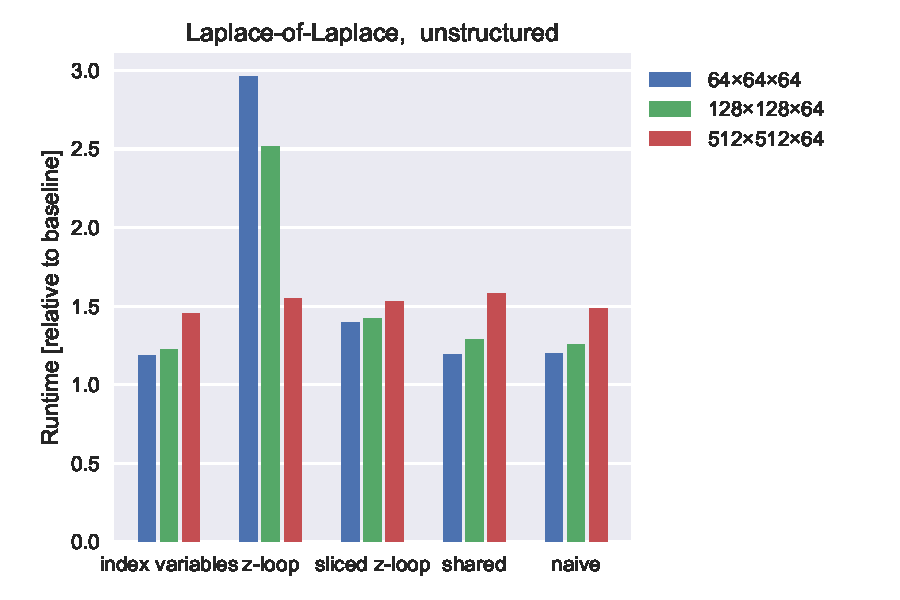
\includegraphics[scale=0.75]{variants-gridsizes.pdf}
	\caption{\label{fig:variants-gridsizes} Relative runtime of different variants of the Laplace-of-Laplace benchmark at different X-Y-sizes with respect to the fastest regular variant. For each bar, the fastest storage variant is considered (fastest of compression/chasing/z-curves). Baseline: fastest regular grid implementation.}
\end{figure}

We have evaluated combinations of grid storage and access variants for the three stencils on grids of X-Y size $64\times 64$ (small grid), $128\times 128$ (medium grid) and $512\times 512$ (large grid). Naturally, larger problem sizes lead to longer run times in all variants. More intrestingly however, increases in the X-Y-domain size affect the unstructured variants more negatively than the regular ones.

For small domains, the runtimes of unstructured variants are generally close to those of their regular counterparts. With increased domain size, there is an increase in the relative slowdown of the unstructured variant with respect to the fastest regular implementation. We assume this is due to cache sizes; while in smaller grids, entire neighborship tables and cell values remain cached, larger grids necessitate larger neighborship tables which cannot fit into the cache together with the cell values as a whole. Figure \ref{fig:variants-gridsizes} shows this trend for the Laplace-of-Laplace benchmark, but the same characteristics apply to the other stencils as well.

The \emph{z-loop} grid access variant is the only exception to the described charateristics. Its relative slowdown decreases for larger grid sizes. This is probably due to two reasons. First, the z-loop variants already suffer from low occupancy in large grids. In small grids, occupancy is even lower, not making use of the complete parallelism capabilities of the GPU. Second, in small grids, the neighborship table may be in cache in its entirety after one read. This allows subsequent neighborship table accesses to be practically free. This offsets the supposed optimization of the z-loop variant, which aims to reduce the number of reads of neighborship table entries. This optimization only begins to provide a benefit in large grids.

\subsection{Change in Z domain size}
\label{sec:res-z-size-change}

\begin{figure}
	% dat = pd.read_csv("results/ultimate-reformat.csv")
	% dat["rel"] = u.relmingroup(dat, by=u.col.stencil+u.col.size)
	% u.lineplot(dat[(dat["stencil"]=="laplap")&(dat["variant"]=="idxvar")&dat["z-curves"]], x="size-z", y="rel")
% fig=u.plotdone(legend=0)
	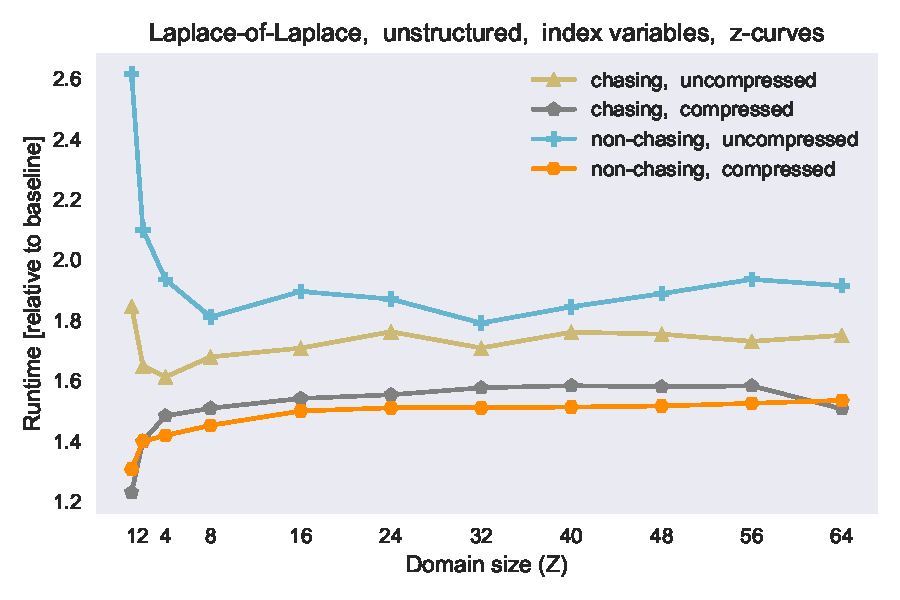
\includegraphics[scale=0.75]{laplap-idxvar-z-sizes.pdf}
	\caption{\label{fig:laplap-z-sizes} Relative slowdowns of the Laplace-of-Laplace stencil on unstructured grids of various Z-sizes. Baseline: fastest regular grid implementation.}
\end{figure}

Given a $512\times 512$ base grid, we benchmarked our stencils with various Z-sizes ranging from $1$ to $64$. We analyzed the cost of using an unstructured grid relative to a regular grid, and observe two main patterns. Which pattern the relative costs follow depends on the chosen grid storage. Figure \ref{fig:laplap-z-sizes} plots the relative slowdowns as a function of the Z-size for the \emph{laplap} stencil using the \emph{idxvar} access method. The plot is roughly representative of all other stencils and access methods. The observed patterns are as follows:

First, for uncompressed storage, the overhead decreases quickly for the first few Z-size steps, then fluctuates around some constant. This can be most clearly be seen in the \emph{non-chasing} stored grids. Second, when compression is used, the overhead increases in the first few Z-size steps, then also remains roughly constant.

These trends can be explained by two countering effects:

On one hand, the increased number of Z-levels obviously results in an increased total number of cells. In an unstructured grid, for each of those cells, some extra effort has to be made to determine the location of the cell's neighbors. We call this the \emph{once-per-cell cost}. This effect alone would lead to constant additional relative costs (linear additional absolute costs) with respect to the regular grid.

On the other hand, as our grids are regular in the Z-dimension, neighborship pointers can be re-used among threads operating on cells with the same X- and Y-coordinates. Let us call a set of cells with identical X- and Y-coordinates a \emph{pillar of cells}. If neighborship pointers are effectively reused, loading them is only a \emph{once-per-pillar} cost. No matter how many Z-levels there are in the grid, the first load of the neighborhip pointers remains a constant cost. As Z-size increases, this constant becomes vanishingly small in relation to the overall cost of the regular-grid computation. Thus, considering only the \emph{once-per-pillar} costs, performance should approach regular grid performance asymptotically for increasing Z. 

The observed relative overheads result from a combination of the two described effects (\emph{once-per-cell} and \emph{once-per-pillar} costs). In the uncompressed variants, the \emph{once-per-pillar costs} appear to dominate; thus, an increase in Z-size leads to better relative runtimes. One could say the ``investment'' of loading the neighborship pointers pays off once they can be reused more often (larger Z-sizes).

Our optimized access strategies aim to make explicit use of the \emph{once-per-pillar} nature of neighborship reads (\emph{shared}, \emph{z-loop} and \emph{z-loop-sliced}). Even the access strategies that do not explicitly exploit Z-regularity benefit from it if neighborship pointers happen to reside in caches (which they most likely will for adequate block sizes due to their frequency of use).  In the best-case scenario, all neighborship pointers are already in L1 cache (\emph{idxvar}), shared memory (\emph{shared} access strategy) or loaded into registers at the beginning of a loop (\emph{z-loop}) when a thread begins computation.

\subsection{Effect of Floating Point Precision}

We observed no significant differences in the relative slowdown when using single-precision floating point data types instead of double-precision data types. As expected, the absolute runtimes decrease with lower precision. This happens in the same proportions for both regular grid and unstructured grid implementations -- both are roughly $40\%$ faster than double-precision speeds.

As it appears to have no effect on the characteristics of our benchmarks, we consistently used double precision data types in all other experiments apart from this section.
\section{Effect of Grid Storage} \label{sec:res-storage}

In section \ref{sec:grid-implementations}, we described different approaches to storing an unstructured grid. Four storage approaches were benchmarked as a result of varying the following two properties: First, the depth of the neighborship table, i.e. whether only neighbors (\emph{chasing} variant) or also neighbors-of-neighbors (\emph{non-chasing} variant) were stored. Second, whether the neighborship table was \emph{compressed} or \emph{uncompressed}.

\begin{figure}
	% ax=u.barplot(df64mins[(df64mins["stencil"]=="hdiff")&df64mins["z-curves"]&(df64mins["size-x"]>=128)], grp=u.col.stencil+u.col.size, cat=u.col.storage, tickrot=0, y="rel")
	% ax.set_ylim(bottom=1)
	% fig=u.plotdone()
	% u.plotsave("report/img/hdiff-z-curves-sizes-storage.pdf", fig)
	\comment{
	      stencil  size-x  size-y  size-z  unstructured        variant  z-curves  no-chase   comp  threads-x  threads-y  threads-z       min       max       avg    median
	11327   hdiff     128     128      64          True         idxvar      True     False  False         64          1          8   50000.0   53000.0   51000.0   51000.0
	12079   hdiff     128     128      64          True         idxvar      True     False   True         32          1         16   52000.0   56000.0   53000.0   53000.0
	10516   hdiff     128     128      64          True         idxvar      True      True  False         32          2          8   47000.0   50000.0   48000.0   49000.0
	10880   hdiff     128     128      64          True          naive      True      True   True         32          1          8   48000.0   51000.0   50000.0   50000.0
	32073   hdiff     512     512      64          True         idxvar      True     False  False         64          1          8  801000.0  828000.0  817000.0  820000.0
	31623   hdiff     512     512      64          True         idxvar      True     False   True        128          1          2  734000.0  746000.0  741000.0  741000.0
	32178   hdiff     512     512      64          True  idxvar-shared      True      True  False         32          1         16  819000.0  854000.0  838000.0  841000.0
	31541   hdiff     512     512      64          True          naive      True      True   True        128          1          2  707000.0  721000.0  713000.0  710000.0
	}
	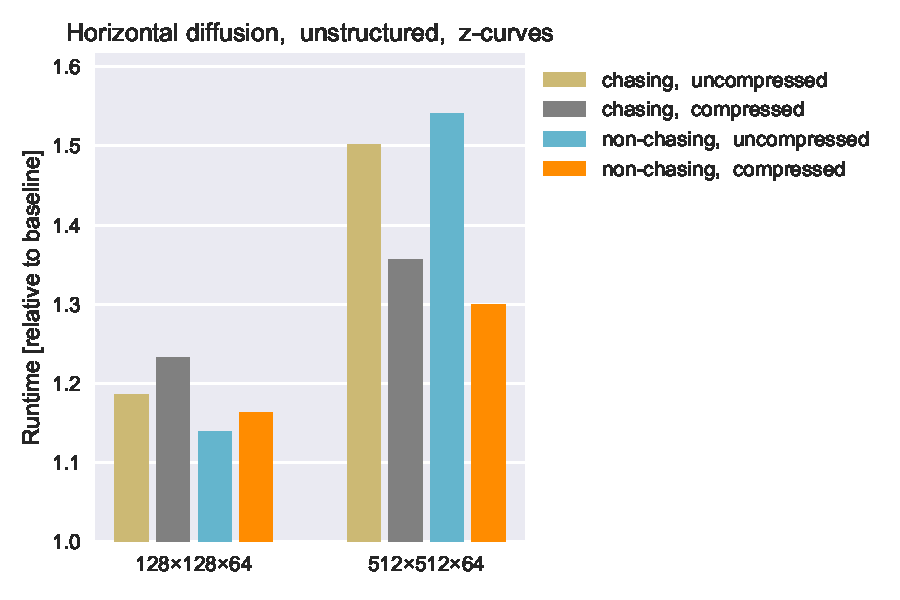
\includegraphics[scale=0.75]{hdiff-z-curves-sizes-storage.pdf}
	\caption{\ref{fig:hdiff-sizes-storage} Relative slowdowns for the horizontal diffusion stencil on a small and a larger grid. The fastest access variant is plotted for each bar, which is one of \emph{index variables}, \emph{naive} and \emph{idxvar-shared} for the shown benchmarks. This example for the horizontal diffusion stencil is representative for the other two benchmarks as well, where the slowdowns follow a similar pattern. (Note that in the fastwaves stencils, pointer chasing is not applicable as there only direct neighbors are accessed.)}
\end{figure}

\subsection{Pointer Chasing versus Explicit Neighbor-of-Neighbor Storage}
\label{sec:results-chasing}

Two of the three benchmarked stencils, Laplace-of-Laplace and Horizontal Diffusion, access neighbors beyond the directly face-touching cells (neighbors of neighbors). For those stencils, two implementations were benchmarked: First, we assessed the performance when only direct neighbors are explicitly stored. This approach requires \emph{pointer chasing}: In order to access the neighbor of a neighbor, two sequential lookups become necessary. As the second lookup can only be started when the first one completed, a higher latency may occur in this variant. Therefore, we then also tested variants in which the neighbors-of-neighbors were explicitly stored in memory, reducing the number of required memory lookups for those cells from two to one. This comes at the cost of a higher memory footprint, however.

Generally we observe the following trend: If the grid is small or compressed, pointer chasing becomes an issue (and thus non-chasing variants profit). In larger uncompressed grids, the latency of the two lookups required in pointer chasing for neighbors-of-neighbors can be effectively hidden. This is visible in figure \ref{fig:hdiff-sizes-storage}, which outlines the differences of the storage approaches for the fastest respective variant of the horizontal diffusion stencil on grids of different sizes. 

In all cases a higher total number of device memory and L2 cache reads is observed in the \texttt{nvprof} metrics for the non-chasing variants. This is to be expected, as non-chasing variants need to store and read more information from a larger number of different addresses. The L1 cache hit rate lowers by around $6\%$ in both large and small grids when pointers to neighbors-of-neighbors are explicitly stored. In large grids, the L2 cache hit rate also drops dramatically; for smaller grids, it is unaffected and remains high. Thus, the additional neighbor-of-neighbor information stored hurts cache locality more in larger grids, putting non-chasing variants at a disadvantage there. This is due to the fact that larger grids require more of this information, while the cache size remains constant -- consequently, some data has to be evicted from the cache. This does not happen as often in a smaller grid. The variants that perform pointer chasing experience a higher percentage of stalls due to memory dependencies due to the second lookup depending on the result of the first for neighbor-of-neighbor reads.  We conclude that non-chasing storage is beneficial to small grids, where it is effective in reducing latency, and unfavorable for larger grids due to the caused cache evictions (especially in the L2 cache), that actually increase the latency of neighbor acceses. Table \ref{tab:chasing} shows an overview of the metrics discussed in this paragraph for an exemplary stencil configuration of the horizontal diffusion stencil.

\begin{table}
	\comment{chase-v-no-chase.txt}
	\begin{tabular}{l l l l l l}
		\hline
		\textbf{Size} & \textbf{Chasing?} & \textbf{\texttt{tex\_cache\_hit\_rate}} & \textbf{\texttt{l2\_tex\_hit\_rate}} & \textbf{\texttt{stall\_memory\_dependency}} & \textbf{Runtime} \\
		\hline
		$128\times 128\times 64$ & - & 			$73\%$ & $68\%$ & $59\%$ & $\mu s$ \\
		$128\times 128\times 64$ & \checkmark & $67\%$ & $72\%$ & $54\%$ & $\mu s$ \\
		$512\times 512\times 64$ & - & 			$68\%$ & $58\%$ & $74\%$ & $\mu s$ \\
		$512\times 512\times 64$ & \checkmark & $63\%$ & $37\%$ & $60\%$ & $\mu s$ \\
		\hline
	\end{tabular}
	\caption{\label{tab:chasing} Selected metrics for runs of the horizontal diffusion stencil on different types of grids (all of them in z-curves layout). The fastest found variant and launch configuration was chosen for each configuration seperately.}
\end{table}

\subsection{Advantage of Compressed Neighborship Tables}

Across all stenils except fastwaves, and across all access implementations, compressing the neighborship table improves performance for large enough grids. Table \ref{tab:compression} shows the distribution of neighborship table entries attained by the trivial compression scheme that we implemented is on a $512\times 512\times 64$-sized grid. If the values of the grid are laid out in row-major fashion, compression is especially effective. In this case, only the elements in the halo have different neighborship pointers; all others share the top entry. Using a z-curves layout, the distribution of neighborship table accesses is more evenly spread out. However, the concentration of several frequently occuring patterns is still able to provide a runtime benefit.

\begin{table}
	\begin{tabular}{l l l l l l}
		\hline
		Compressed? & Chasing? & Storage & \# Entries & Ratio\textsuperscript{*} & Freq.\textsuperscript{\dag} \\
		\hline
		- & \checkmark & both & $1,048,576$ & $1$ & $<1\%$\\
		- & - & both & $3,145,728$ & $1$ & $<1\%$\\
		\checkmark & \checkmark & row-major & $2054$ & $0.00078$ & $97.7\%$ \\
		\checkmark & \checkmark & z-curves & $2435$ & $0.00093$ & $20.3\%$ \\
		\checkmark & - & row-major & $4093$ & $0.00156$ & $96.9\%$ \\
		\checkmark & - & z-curves & $5299$ & $0.00202$ & $8.1\%$ \\
		\hline
	\end{tabular}
	\caption{\label{tab:compression} Properties of neighborship table before and after compression for different types of grids. \textsuperscript{*}Ratio of number of compressed neighborship table entries to number of uncompressed neighborship table entries. \textsuperscript{\dag}The frequency given is the frequency of the most common neighborship table entry. }
\end{table}

\begin{verbatim}
% TODO
% - Relative advantage of compression for all variants/combinations
% - Why not larger advantage? -> Metrics to back up coalescing explanation/latency of first prototype lookup and second lookup is non-coalesced
% - Why uncompressed faster for fastwaves?

% mention fewer memory dram transactions/bytes in compressed variants
% mention higher hit rate for large grids, smaller hit rate for small
\end{verbatim}

\section{Effect of Access Strategy} \label{sec:res-access}

In section \ref{sec:optimizations}, we discussed various optimizations for accessing such grids in a stencil application. Here, we compare the performance of these approaches. Figure \ref{fig:storage-access} gives an overview of the possible storage/access-combinations.

% Idea: percentage effect of access strategy given fixed storage; how important is access strategy?

\subsection{\emph{Naive} and \emph{Idxvar} Access Strategies}
The \emph{naive} and \emph{idxvar} (index variables) access strategies are among the fastest for all three stencils. In some cases, the \emph{naive} access strategy is faster than the \emph{idxvar} variant by a very slight margin. This is the case, for example, in the fastwaves stencil or the horizontal diffusion stencil executed on a non-chasing, compressed grid. This result might appear surprising at first, as the naive strategy repeatedly performs memory lookups for the same neighborship pointers. The index variables approach tries to reduce these reduntant lookups by storing the needed neighborship indices in temproary variables at the start of the kernel execution. However, this adds some overhead.

For one, the index variables variant for the fastwaves kernel leads to a higher register use when compiled (44 registers for \emph{idxvar} versus 42 for \emph{naive}). As registers are shared across threads of a block, this reduces the theoretical amount of threads that can be launched concurrently. As this difference is not present in the other stencils, this does not appear to be the main reason for the advantage, however. There are two more likely explanations for the advatnage of the \emph{naive} variant: First, access to the same memory location in the \emph{naive} kernel becomes as cheap as a register access after a neighborship pointer are read for the first time, as it will be held in the L1 cache. Reaccessing the same memory location helps keep the values fresh in all caches. As such, when a different thread requires the same memory location from the neighborship table, it is more likely to be in cache in the \emph{naive} variant. Second, the naive approach has better \emph{instruction level parallelism}. Because the index variables are assigned at the start of the \emph{idxvar} variant, all loads to the neighborship table are gathered in one sequence and must be executed before anything else. In the \emph{naive} approach, on the other hand, neighborship pointers are (re-)loaded only when needed in calculations. Thus, after one neighbor has been loaded, useful calculations using its value may already be performed. Table \ref{tab:fastwaves-naive-idxvar-metrics} details profiler metrics that support these claims.

\begin{table}
	\begin{tabular}{l l l}
		\hline
		Metric & \emph{naive} & \emph{idxvar} \\
		\hline
		Run time & $\mathbf{2438\mu s}$ & $2543\mu s$ \\
		Global load transactions & $126264460$ & $124235165$ \\
		L1 transactions & $38077396$ & $34593863$ \\
		L2 transactions & $56635611$ & $57264861$ \\
		Device Memory transactions & $36825619$ & $37327310$ \\
		Executed Instructions Per Cycle & $\textbf{0.522}$ & $0.497$ \\
		\hline
	\end{tabular}
	\caption{\label{tab:fastwaves-naive-idxvar-metrics}Selection of metrics for \emph{fastwaves} stencil run on a $512\times 512\times 1$-sized unstructured grid (z-curves layout, compressed neighborship table) with $32\times 1\times 8$ threads, which is the fastest block size for both variants. The \emph{naive} implementation is faster, even though it redoes the index lookups in the neighborship tables. The total global transaction count shows that the \emph{idxvar} variant successfully reduces the number of neighborship lookups performed. However, the cache transactions (L1 and L2) indicate that the naive variant keeps cache contents fresher and results in more cache hits. This is evidenced by the lower number of actual device memory reads in the naive approach, despite the idxvar approach requesting less memory.}
\end{table}

% main advantage idxvar vs naive: all neighbor pointers loaded together in the beginning; for non-chasing this is a disadvantage (all accesses bundled together; with naive some things can happen in between while load is happening); for chasing an advantage for idxvar (first load all level-one pointers, then all level two; re-loading all of this is costly for naive but has to be done because it can't know the first pointer hasn't changed in the meantime)

\subsection{\emph{Shared} Access Strategy}

The performance of the \emph{shared} access strategy varies strongly depending on the storage strategy -- specifically, whether compression for the neighborship tables is used or not.

In all scenarios with uncompressed neighborship stroage, the \emph{shared} access strategy performs almost identically to the \emph{idxvar} access strategy. A very slight overhead is observed for the \emph{shared} access strategy due to the required thread synchronizations. The neighborship pointers loaded into shared memory appear to take the same role as the L1 cache in the \emph{idxvar} strategy. Thus, the \emph{shared} access strategy can be viewed as an \emph{explicitly managed cache}. In fact, as mentioned in section \ref{sec:memories}, shared memory and L1 cache share the same physical memory. Table \ref{tab:access-shared} further evidences how the L1 cache is simply shifted to shared memory in this access strategy.

The z-curves, non-chasing and non-compressed storage strategy stands out in the shared access strategy, as this is the only configuration in which the \emph{shared} access strategy slightly outperforms the \emph{idxvar} access strategy. In the aforementioned storage configuration, an explicit management of unified L1/shared appears provides a very slight benefit. This is probably due to the very large number of neighbor pointers in this storage strategy.

When using compressed neighborship tables, the \emph{shared} access strategy is noticeably slower than the \emph{idxvar} strategy. As there are relatively few neighborship pointers in compressed tables, those remain in \emph{L1} cache in the \emph{idxvar} variant permanently. In the \emph{shared} variant, those same (few) pointer(s) are (re-)loaded into shared memory for each thread block, which is less efficient.

\begin{table}
	% ==20891== Profiling application: ./gridbenchmark --no-verify --size 512x512x64 --threads 64x1x8 hdiff-unstr-idxvar -z hdiff-unstr-idxvar-shared -z
	%    Kernel: void HdiffCudaUnstr::Chasing::hdiff_idxvar<double>(_coord3<int>, int const *, int, int, double const *, int const **, double const )
%         21                    tex_cache_transactions   Unified cache to Multiprocessor transactions    29954766    29968023    29962684
%         21                  l2_tex_read_transactions                L2 Transactions (Texture Reads)    22371588    22389494    22381872
%         21                  shared_load_transactions                       Shared Load Transactions           0           0           0
%         21                        tex_cache_hit_rate                         Unified Cache Hit Rate      72.14%      72.16%      72.15%
%         21                           l2_tex_hit_rate                              L2 Cache Hit Rate      50.48%      50.56%      50.53%
%         21                    dram_read_transactions                Device Memory Read Transactions     9358879     9369522     9362526
%    Kernel: void HdiffCudaUnstr::Chasing::hdiff_idxvar_shared<double>(_coord3<int>, int const *, int, int, double const *, int const **, double const )
%         21                    tex_cache_transactions   Unified cache to Multiprocessor transactions    26586311    26591481    26589268
%         21                  l2_tex_read_transactions                L2 Transactions (Texture Reads)    22323586    22341588    22333518
%         21                  shared_load_transactions                       Shared Load Transactions     5661664     5674694     5666573
%         21                        tex_cache_hit_rate                         Unified Cache Hit Rate      62.35%      62.38%      62.36%
%         21                           l2_tex_hit_rate                              L2 Cache Hit Rate      50.55%      50.63%      50.59%
%         21                    dram_read_transactions                Device Memory Read Transactions     9353607     9360039     9355089
	\begin{tabular}{l l l}
		\hline
		Metric & \textbf{\emph{idxvar}} & \textbf{\emph{shared}} \\
		\hline
		L1 Cache Transactions & $29,962,684$ & $26,589,268$ \\
		Shared Mem. Transactions & $0$ & $5,666,573$ \\
		DRAM Reads & $9,362,526$ & $9,355,089$ \\
		\hline
	\end{tabular}
	\caption{\label{tab:access-shared} Number of transactions per access strategy at various levels of the memory hierarchy for a benchmark of the \emph{Horizontal Diffusion} stencil (grid of size $512\times 512\times 64$, z-curves, pointer chasing, uncompressed) at $64\times 1\times 8$ threads per block (optimal for both access strategies). A number of L1 cache hits in the \emph{idxvar} strategy are simply shifted to equally performant shared memory hits in the \emph{shared} strategy. The number of reads encountered at device memory is similar, further indicating that shared memory usage simply serves as a explicit, manually managed cache, taking the same role as the L1 cache in the \emph{idxvar} access strategy.}
\end{table}

% almost identical to idxvar for most storage strategies -> explicit cache management vs default idxvar cache TODO metrics shared memory accesses ~=~ cache hits?

% z-curves, non-chasing, uncompressed -> shared very slightly faster (there are really many neighborship pointers and explicitly using cache makes sense here (not enough reuse to make automatic cache useful))

% worse for compressed storage -> overhead of explicit shared memory management, possibly less efficient manual allocation?


\subsection{\emph{Z-loop} and \emph{Z-loop-sliced} Access Strategies}

For the \emph{hdiff} and \emph{fastwaves} stencils, the two \emph{z-loop} access strategies performed noticeably slower than the other available access strategies, across all tested grid storage configurations. The same was the case for the \emph{laplap} stencil for compressed grids. The one exception is the \emph{laplap} stencil on an uncompressed grid: In this case the \emph{z-loop} access strategy was the fastest.

The anticipated advantage of the two \emph{z-loop} access strategies is the reduced number of required neighborship table reads. Indeed, the number of reads to device memory is greatly reduced using this access strategy in all stencils (more than halved for \emph{laplap}, $56\%$ for \emph{hdiff}). In the case of the computationally simple \emph{laplap} stencil on an uncompressed grid, this reduced number of reads pays its dividends; the \emph{z-loop} access strategy is the fastest for this specific benchmark.

For other stencils (and the \emph{laplap} stencil in compressed grids), using the \emph{z-loop} access strategy is slower than all the alternatives.  We assume that this is due to the much lower (compared to other access strategies) occupancy of this loop-based access strategy. In the more computationally complex stencils, more latencies in the result computations may occur, which require a large number of threads to hide. In the \emph{z-loop} access strategy, a sequential processing of all elements with the same X- and Y-coordinates is prescribed by the code -- hindering parallel execution on the GPU. Presumably, this is less of an issue in the \emph{laplap} stencil due to its more simplistic result computation and fewer fields, which leads to fewer stalls in need of latency hiding.

The \emph{z-loop-sliced} variant tries to address some of the low-occupancy issues by splitting the loop into smaller, parallelizable chunks. The idea is to get the best of both worlds: Reuse of neighborship table reads in a loop and more parallelism thanks to more threads. While the performance does improve in comparison with the \emph{z-loop} access strategy (confirming our theory that occupancy is indeed the bottleneck), it still falls short of the other access strategies.

Table \ref{tab:access-z-loop} shows the relevant metrics of the described observations for an exemplary benchmark run.

\begin{table}
	\begin{tabular}{l l p{2.5cm} p{2.5cm} p{2.5cm}}
		\hline
		\textbf{Stencil} & \textbf{Access} & \textbf{\texttt{achieved\_\allowbreak occupancy}} & \textbf{\texttt{ipc}} & \textbf{\texttt{dram\_\allowbreak read\_\allowbreak transactions}} \\
		\hline
		\hline
		\emph{laplap} & \emph{idxvar} & $0.947077$ & $0.812799$ & $11,946,136$ \\
		& \emph{z-loop} & $0.407226$ & $0.515881$ & $4,715,455$ \\
		& \emph{z-loop-sliced} & $0.421727$ & $0.638366$ & $4,729,444$ \\
		\hline
		\emph{hdiff} & \emph{idxvar} & $0.935448$ & $0.793701$ & $16,606,211$ \\
		& \emph{z-loop} & $0.363111$ & $0.481847$ & $9,330,226$ \\
		& \emph{z-loop-sliced} & $0.301747$ & $0.600179$ & $9,354,882$ \\
		\hline
	\end{tabular}
	\caption{\label{tab:access-z-loop} Relevant metrics for comparison of \emph{z-loop} and \emph{idxvar} access strategies on two stencils, on a $512\times 512\times 64$-sized grid (uncompressed, pointer chasing, z-curves layout) with $64\times 2\times 1$ threads.}
\end{table}

% As with the \emph{shared} access strategy, the two \emph{z-loop} strategies aim to improve performance by maximizing the use of a cell's neighborship pointers once they have been loaded. Instead of performing only the output calculation for one cell, the result for cells of all Z-levels (a set of 8 threads in the \emph{z-loop-sliced} variant) are computed.

% + laplap, uncompressed (fastest!)
% - hdiff, fastwaves (low occupancy maybe? -> hdiff more compute expensive w branches)

% This optimization does reduce the number of reads to the neighborship tables. However, once the neighborship pointers are loaded into L1 and L2 caches,  re-reads of the same neighborship pointers complete in the same order of magnitude as register reads.

% ==13459== Profiling application: ./gridbenchmark --size 512x512x64 --no-verify --threads 64x2x1 hdiff-unstr-idxvar-kloop laplap-unstr-idxvar-kloop hdiff-unstr-idxvar laplap-unstr-idxvar
% ==13459== Profiling result:
% ==13459== Metric result:
% Invocations                               Metric Name                           Metric Description         Min         Max         Avg
% Device "Tesla V100-PCIE-32GB (0)"
%     Kernel: void HdiffCudaUnstr::Chasing::hdiff_idxvar<double>(_coord3<int>, int const *, int, int, double const *, int const **, double const )
%          21                        achieved_occupancy                           Achieved Occupancy    0.934729    0.936472    0.935356
%          21                                       ipc                                 Executed IPC    0.754605    0.806749    0.791383
%          21                    issue_slot_utilization                       Issue Slot Utilization      18.87%      20.17%      19.79%
%          21                     stall_exec_dependency   Issue Stall Reasons (Execution Dependency)       4.67%       5.05%       4.95%
%          21                    dram_read_transactions              Device Memory Read Transactions    16579735    16691044    16608391
%     Kernel: void HdiffCudaUnstr::Chasing::hdiff_idxvar_kloop<double>(_coord3<int>, int const *, int, int, double const *, int const **, double const )
%          21                        achieved_occupancy                           Achieved Occupancy    0.360505    0.366742    0.363722
%          21                                       ipc                                 Executed IPC    0.423041    0.505123    0.483726
%          21                    issue_slot_utilization                       Issue Slot Utilization      10.58%      12.63%      12.10%
%          21                     stall_exec_dependency   Issue Stall Reasons (Execution Dependency)       6.46%       7.39%       7.06%
%          21                    dram_read_transactions              Device Memory Read Transactions     9195785     9933908     9352489
%     Kernel: void LapLapUnstr::Chasing::laplap_idxvar_kloop<double>(int const *, int, int, _coord3<int>, double const *, _coord3<int>*)
%          21                        achieved_occupancy                           Achieved Occupancy    0.402836    0.410686    0.407008
%          21                                       ipc                                 Executed IPC    0.488878    0.584792    0.522810
%          21                    issue_slot_utilization                       Issue Slot Utilization      12.22%      14.62%      13.07%
%          21                     stall_exec_dependency   Issue Stall Reasons (Execution Dependency)       5.71%       6.69%       6.06%
%          21                    dram_read_transactions              Device Memory Read Transactions     4577237     4805963     4702576
%     Kernel: void LapLapUnstr::Chasing::laplap_idxvar<double>(int const *, int, int, _coord3<int>, double const *, _coord3<int>*)
%          21                        achieved_occupancy                           Achieved Occupancy    0.946763    0.947602    0.947077
%          21                                       ipc                                 Executed IPC    0.805199    0.818363    0.812799
%          21                    issue_slot_utilization                       Issue Slot Utilization      20.13%      20.46%      20.32%
%          21                     stall_exec_dependency   Issue Stall Reasons (Execution Dependency)       5.11%       5.20%       5.16%
%          21                    dram_read_transactions              Device Memory Read Transactions    11926443    12023609    11946136

\section{Conclusions}

\printbibliography

\end{document}
